% Compile with pdfLaTeX twice: pdflatex report.tex
% Submitted report wording is preserved. See ../Content_Preservation_Audit.txt.
\documentclass[11pt,a4paper,onecolumn]{article}
\usepackage[margin=21mm,top=20mm,bottom=20mm]{geometry}
\usepackage[T1]{fontenc}
\usepackage[utf8]{inputenc}
\usepackage{tgtermes,mathptmx}
\usepackage{amsmath,amssymb}
\usepackage{graphicx,longtable,array,booktabs,caption}
\usepackage[table]{xcolor}
\usepackage{microtype,titlesec,needspace}
\usepackage[unicode,hidelinks]{hyperref}
\urlstyle{same}
\hypersetup{pdftitle={Bubble Detection and Dating in Fan Tokens},pdfauthor={FRAM Group G07}}
\setlength{\parindent}{0pt}
\setlength{\parskip}{6pt plus 1pt minus 1pt}
\linespread{1.10}
\setcounter{secnumdepth}{0}
\titleformat{\section}{\large\bfseries}{}{0pt}{}
\titleformat{\subsection}{\normalsize\bfseries}{}{0pt}{}
\titleformat{\subsubsection}{\normalsize\bfseries}{}{0pt}{}
\titlespacing*{\section}{0pt}{13pt}{5pt}
\titlespacing*{\subsection}{0pt}{10pt}{4pt}
\titlespacing*{\subsubsection}{0pt}{9pt}{4pt}
\captionsetup{font=small,labelformat=empty,justification=raggedright,singlelinecheck=false,hypcap=false}
\setlength{\emergencystretch}{2em}
\widowpenalty=10000
\clubpenalty=10000
\raggedbottom
\newcommand{\reportcaption}[1]{{\small\raggedright #1\par}\nopagebreak\vspace{3pt}}
\newenvironment{reportreference}{\begingroup\small\setlength{\parskip}{5pt}\leftskip=5mm\parindent=-5mm}{\par\endgroup}
\begin{document}

{\LARGE\bfseries Bubble Detection and Dating in Fan Tokens: A SADF/BSADF, Change-Point and Bayesian Time-Series Analysis\par}\vspace{6pt}

{\small FRAM Group G07\\29 October 2026\par}\vspace{6pt}

\subsection{Abstract}

The general trend observed across the results is that price deviations tend to reinforce themselves within a given period, this observation is supported across several fan tokens. Through 30 June 2026 , 9 /20 (45\%) of the studied tokens exceeded the 5\% GSADF reference threshold, however none stayed above the dating threshold for the 30 days required to count as an episode. In summation the results imply intermittent explosive behavior and high yet constantly changing volatility rather than widespread, sustained bubbles.

\section{1 Introduction}

The rapid adoption of cryptocurrencies such as Bitcoin, Ethereum, Tether, etc. is a direct result of the rising demand from investors to shift away from currencies that may be influenced by central banks and governments towards a type of currency over which they hold greater ownership and control. Noting the potential growth of cryptocurrency as a niche, businesses have also started issuing cryptocurrencies as a means of raising funds while providing investors with a variety of perks that may or may not be strictly monetary. Fan tokens are one such example. They were initially introduced by Juventus Football Club through the launch of “\$JUV”, which gave holders access to a variety of fan-related membership perks such as voting on club decisions, rewards, and merchandise designs. Fan tokens act as blockchain-based digital assets that may be issued by entertainment entities such as sports clubs, production studios, individual actors, etc., for the purpose of raising funds from fans. They are usually distributed and traded through dedicated platforms such as Chiliz/Socios. The rise of fan tokens is majorly attributed as an attempt by clubs to convert fan loyalty and engagement into a tradable digital instrument, extending traditional membership and merchandising relationships into a new asset form (Ante et al., 2023).

 The prices of fan tokens are much more responsive to the influence of external events, such as match results, transfer news, trophy wins, etc., compared to conventional equity and debt instruments. This can lead to fan-token prices becoming divorced from the actual fundamental value of the clubs associated with them.The study Detecting and Analyzing Explosive Bubbles and Their Relationship with Volatility: Evidence from Tunisia (Ben Yaala \& Henchiri, 2025) suggests that during active bubble phases, heavy retail or institutional participation, such as that seen during crypto or technology-sector manias, can drive up return dispersion and cause rapid price swings. Upon reading such studies, an investor may begin to question the possibility that fan tokens, and cryptocurrencies as a whole, may be forming a bubble. However, it is important to note that volatility alone does not establish the existence of a financial bubble. 

A financial bubble can generally be understood as a period during which an asset's price rises explosively, often driven by speculative demand and expectations of further appreciation rather than changes in fundamentals, before eventually correcting (Kindleberger, 1978; Kindleberger \& Aliber, 2005).Bubble behaviour may arise from financial, economic, and, more broadly, psychological factors. Since, in an efficient market, no asset should be valued differently from its fundamental value, speculative mispricing, which is commonly observed in fan tokens, can expose investors to abrupt price corrections.

A commonly used method for identifying periods of explosive price behavior is based on the augmented Dickey–Fuller (ADF) test. By applying the ADF test recursively, the approach examines whether a time series exhibits a mildly explosive root (Phillips et al., 2011).Supremum ADF( SADF) is a recursive extension of the ADF. It is a statistic obtained by recursively applying the ADF test and taking the supremum (maximum) of the resulting values. SADF thus was mainly developed for detecting whether explosive behavior occurred within some point in the sample rather than identifying the timing of individual episodes.

Explosive-root testing has some limitations. It primarily focuses on identifying periods of explosive behavior in a price series. It thus fails to acknowledge other structural changes in behavior like volatility,persistence and trend, which by themselves do not indicate explosive behaviour but may definitely influence the explosive episodes and their occurrence. Change-point approaches provide a framework for identifying structural changes or regime shifts within a time series (Bai \& Perron, 1998, 2003; Killick et al., 2012). It can be used to find the points where any of the statistical behaviour like trend or volatility or persistence changes.

\section{2 Literature review}

\subsection{2.1 Fan-token utility and speculative value}

Fan tokens are blockchain-based digital assets issued by a sports club which provide small-scale governance and engagement benefits with speculative characteristics. They provide no equity, no dividend or no claim on club earnings but may offer voting rights, rewards, and exclusive content (Ante et al., 2024a, 2025). Cong et al. (2021) implies that the value of tokens arises from transaction demand, network adoption, platform productivity, and expected growth, instead of cash flows and potentially generate appreciation and bubble-like dynamics. While, gamification and tradability of the tokens may encourage gambling-like behaviour by combining limited utility provided by the tokens with speculative trading which can create risks for younger and inexperienced fans (Lopez-Gonzalez and Griffiths, 2023). Fan tokens are also highly volatile, closely connected to cryptocurrencies, and generally underperform the benchmarks over long time periods. (Scharnowski et al., 2023; Vidal-Tomás, 2024).

\subsection{2.2 Impact of sporting information on price formation}

Sporting results become a fundamental source of price changes. For example, Champions League victories produced positive abnormal returns, while defeats created larger negative market reactions (Demir et al., 2022). Trading in fan tokens often rises roughly six months before matches, followed by declining returns and trading volumes during or afterwards. Defeats in high stake matches showed more volatility in returns as compared to that after defeats in low stake matches as seen around the 2022 World Cup, particularly after unexpected knockout defeats (Ante et al., 2024b; Saggu et al., 2024). While injuries, player transfers, shifting sentiment, and market conditions heavily influence prices, event studies are not able to  establish whether sporting news begins, ends, or occurs within a bubble. (Agnese \& Xiao, 2025; Blom \& Henriques Pereira, 2026; Luo et al., 2026).

\subsection{2.3 Attention, behaviour, and market transmission}

Behavioural factors such as the fear of missing out, herding, loss aversion, and overconfidence increase cryptocurrency investment intentions (Kaur et al., 2024). Probability of an asset entering a bubble is largely associated with search activity, trading volume, and social-media attention (Enoksen et al., 2020; Shahzad et al., 2022; Haykir and Yagli, 2022). It is thus evident that volatility alone is not evidence of a bubble because empirical evidence shows that many cryptocurrency bubble days occur during low-volatility regimes (Diniz et al., 2023).

\subsection{2.4 Bubble detection and methodological reliability}

Phillips et al. (2011, 2015a, 2015b) developed recursive right-tailed unit-root tests for detecting explosive market behaviour. GSADF tests for multiple episodes, while BSADF estimates their beginning and end dates. On applying these methods, it was found that fan-token market is highly prone to bubbling. For example, explosivity in 13 of the 20 largest fan tokens (Assaf et al., 2024) and multiple bubbles and collapses in a fan-token index and Chiliz (Vidal-Tomás, 2024). However, short trading history, changing volatility, and serial dependence can produce unreliable dates. Wild-bootstrap, volatility-rescaled, and dependence-robust procedures improve inference (Harvey et al., 2016, 2025; Lui et al., 2024). Structural-break and Bayesian change-point methods can assess whether detected episodes coincide with regime changes. Combining these approaches provides a credible framework for identifying and interpreting fan-token bubbles.

\subsection{2.5 Research Gap}

\subsubsection{2.5.1 Lack of Robust Bubble Testing Under Changing Volatility}

Research by Assaf, Demir, and Ersan (2024) focusing on descriptive analysis observe extreme right-skew and unusually high kurtosis in fan-token prices (e.g., ATM and JUV exceed a kurtosis of 11). Assaf et al explicitly cite Harvey, Leybourne, Sollis, and Taylor (2016) as motivation for wild-bootstrap critical values, Despite citing this methodological concern, Assaf et al. use classical Monte Carlo critical values for their primary GSADF analysis. Harvey et al. (2016) demonstrate analytically that the standard SADF/GSADF statistic "can be severely oversized" under this class of non-stationary-volatility data-generating process, with a corresponding "higher than expected probability of spurious bubble identification." Harvey, Leybourne, Taylor, and Zu (2025) extend the correction further under a broader heteroskedasticity class, and Lui, Phillips, and Yu (2024) extend robustness to strongly dependent (long-memory) error structures, a plausible feature of thinly traded fan-token series exhibiting return persistence. None of these corrections has been applied to fan-token data. This constitutes a validity gap that existing fan-token bubble counts may be inflated by spurious detections attributable to volatility clustering rather than genuine explosive price behaviour

\subsubsection{2.5.2 Limited Cross-Validation of Bubble Detection Methods}

The Assaf, Demir, and Ersan (2024) study cross-validates GSADF against LPPLS, but LPPLS converges (without becoming trapped in local minima, per Filimonov and Sornette, 2013) for only 10 of 20 tokens, leaving half the sample without independent confirmation. No fan-token study has additionally cross-validated against a Bayesian change-point framework (Thies and Molnár, 2018) or a non-parametric sequential Kolmogorov–Smirnov change-point model (Ross and Adams, 2012; operationalised as KS-CPM in the methodology paper). The absence of this cross-validation leaves open the possibility that GSADF/LPPLS results for fan tokens are method-artefacts rather than robust findings.

\subsubsection{2.5.3 Failure to Distinguish Bubble Life-Cycle Stages}

The GSADF/BSADF procedure of Assaf, Demir, and Ersan (2024) identifies windows such that the price change / movement process is statistically explosive but does not decompose these windows into the formation, burst, and decline phases that both Boubaker, Liu, Sui, and Zhai (2022) and Vriz and Grossi (2026) treat as mutually exclusive yet informative in nature.

\subsubsection{2.5.4 Lack of Testing for Event-Driven Micro-Bubbles}

Sharp, short-horizon fan-token price reactions to sporting events like anticipatory World Cup gains and event-driven reversals (Saggu et al., 2024), intraday reactions to match outcomes (Ante et al., 2024b), and asymmetric reactions to match surprise (Blom and Henriques Pereira, 2026; Demir, Ersan, and Popesko, 2022) affect bubble formation. Yet none of the studies applies a formal explosiveness test to the reaction window they document. It is therefore unknown whether these documented "anticipatory gains" and "event-driven losses" are statistically indistinguishable from noise-driven reversion, or whether they in fact constitute short-lived, sport-event-triggered explosive episodes in the SADF/GSADF.

\subsubsection{2.5.5 Limited Sample Coverage in Bubble Predictor Models}

 Assaf, Demir, and Ersan (2024)’s individual-token probit models are estimable for only 5 of its 20 tokens (those exceeding a 3\%-of-days bubble threshold), and even within this small subsample, predictor signs are inconsistent across tokens (e.g., VIX enters positively for GAL but negatively for CITY and DAVIS). No study has addressed this with a hierarchical or Bayesian pooling approach that could borrow statistical strength across the full, unbalanced 20-token panel rather than discarding 75\% of the sample, a natural role for the Bayesian time-series component of the proposed methodology.

This study aims to address these gaps by distinguishing ordinary volatility from statistically explosive behaviour and combining bubble-detection procedures with change point analysis. This methodology thus aims to provide more reliable estimates of bubble formation and collapse while clarifying whether explosive episodes coincide with changes in the underlying price-generating process.

The literature review and research gaps establish the basis for the study objectives. The following sections carry these objectives into the proposed empirical framework and the description of the fan-token panel.

\section{3 Objectives of the study}

The core objective is to identify date periods when fan tokens exhibit explosive price behaviour in a fixed panel of 20 sports fan tokens, while simultaneously isolating these episodes from baseline cryptocurrency volatility. Recursive right-tailed unit-root tests on daily log prices are implemented allowing the detection of explosive trajectories diverging from martingale dynamics, with backward test statistics establishing the exact start and end dates. Rather than imposing a uniform panel start date that truncates price histories, tokens are added to the dataset based on their first valid trading dates to maintain structural data integrity. Then, the results are checked against market conditions of some key reference cryptocurrencies, namely Bitcoin, Ethereum, and Chiliz (CHZ), to determine whether price surges are isolated to one token, market-wide, or linked to the Chiliz ecosystem.

The statistical reliability of these detected windows is further validated via a sequential Kolmogorov-Smirnov test, which assumes no fixed distribution, and a Bayesian change-point model, ensuring regime shifts reflect genuine distributional variance without making restrictive parametric assumptions. Ultimately, a hierarchical dynamic model combines cross-sectional information across all tokens to see how bubble states interact with lag returns, volatility, trading activity, and overall crypto market moves. This design addresses changing volatility, heavy-tailed return distributions, short price histories, and tokens having different numbers of episodes, thereby, helping label each episode as formation, burst, or decline, instead of just listing bubble dates.

\section{4 Methodology}

\subsection{4.1 Empirical design}

The methodology combines the fan-token framework with an empirical detection and change-point model. In stage 1, we determine explosive behaviour in each individual log-price series. Then, in stage 2, it uses backward recursive statistics to find the exact timestamps of each detected episode. Then in stage 3,  non-parametric and Bayesian change-point methods are used to test whether these episodes coincide with changes in the return distribution. Finally, in stage 4,we estimate a hierarchical Bayesian dynamic model for the bubble indicator in the overall unbalanced panel. The four levels work in concert to address some particular analytical issues, rather than replacing one another.

\par\addvspace{5pt}\noindent\begin{minipage}{\linewidth}\reportcaption{Table 1. Relationship between the empirical methods}

\begingroup\small\renewcommand{\arraystretch}{1.18}\setlength{\tabcolsep}{4pt}\arrayrulecolor{lightgray}
\noindent\begin{tabular}{|>{\raggedright\arraybackslash}p{0.224242\dimexpr\linewidth-6\tabcolsep-4\arrayrulewidth\relax}>{\raggedright\arraybackslash}p{0.321212\dimexpr\linewidth-6\tabcolsep-4\arrayrulewidth\relax}>{\raggedright\arraybackslash}p{0.454545\dimexpr\linewidth-6\tabcolsep-4\arrayrulewidth\relax}|}
\hline\rowcolor[HTML]{E8E8E8} \bfseries Stage & \bfseries Method & \bfseries Primary output \\ \hline
Explosive-root testing & SADF and GSADF & Whether at least one explosive episode exists \\ \hline
Episode dating & BSADF sequence & Start and end dates of explosive windows \\ \hline
Distributional validation & Sequential KS-CPM & Non-parametric changes in the return distribution \\ \hline
Probabilistic validation & Bayesian change points & Posterior probability of regime shifts \\ \hline
Panel explanation & Hierarchical dynamic logit & Shared and token-specific predictors of bubble states \\ \hline
\end{tabular}\endgroup\end{minipage}\par\addvspace{5pt}

\subsection{4.2 Recursive right-tailed ADF tests}

For each token, the tests are estimated on log price because an explosive root is a property of the price level rather than the stationary return series. On a subsample beginning at fraction r1 and ending at fraction r2 of T observations, the augmented Dickey-Fuller regression is:

\[
\Delta y_t=\alpha_{r1,r2}+\beta_{r1,r2}y_{t-1}+\sum_{j=1}^{k}\phi_{j,r1,r2}\Delta y_{t-j}+\varepsilon_t
\]

The right-tailed null and alternative are H0: beta equals zero against H1: beta is greater than zero. The lag order k is selected by the Bayesian information criterion from zero to the Schwert maximum for each token. The minimum window is token-specific and follows the Phillips-Shi-Yu rule below, rounded upward to an integer number of observations.

\[
r_0=0.01+\frac{1.8}{\sqrt{T}}
\]

The SADF statistic fixes the first observation and expands the endpoint, making it useful for detecting a single dominant episode. The GSADF statistic allows both endpoints to vary and is therefore the primary full-sample test when multiple episodes may occur (Phillips, Shi and Yu, 2015a, 2015b).

\[
\mathrm{GSADF}(r_0)=\sup_{r2\in[r0,1],\ r1\in[0,r2-r0]}\mathrm{ADF}_{r1}^{r2}
\]

As the preliminary evidence shows strong volatility clustering, standard Monte Carlo critical values that work with homoskedasticity assumption may give unreliable results. Primary inference will use 999 wild-bootstrap replications with a fixed, recorded seed, so that the results are reproducible. This handles the heteroskedasticity problem documented in Harvey et al. (2016). Sensitivity checks reported along with primary results will include conventional critical values and the volatility-rescaled test of Harvey et al. (2025). If long-memory diagnostics indicate strong dependence, we will apply the self-normalized robust procedure from Lui, Phillips and Yu (2024), and compare the results with the primary inference. 

\subsection{4.3 BSADF date-stamping}

If the null hypothesis of no-explosiveness is rejected, a backward-looking sequence is calculated for every valid endpoint. For any given endpoint r2, the BSADF statistic is the largest right-tailed ADF statistic obtained by varying the starting point across all permissible windows.

\[
\mathrm{BSADF}_{r2}(r_0)=\sup_{r1\in[0,r2-r0]}\mathrm{ADF}_{r1}^{r2}
\]

An episode starts when the BSADF sequence first exceeds its 95\% bootstrap critical value, and ends when the BSADF sequence falls below this threshold. Primary specification requires at least 5 consecutive days to avoid marking isolated one-day crossings as full episodes. Sensitivity checks also test 3-day, 7-day and 14-day minimum-duration rules. Overlapping or adjacent episodes are merged only according to a predefined and well documented rule applied uniformly across all tokens. The output for each asset includes GSADF statistic, p-value, episode start and end dates, episode duration, peak date, maximum price appreciation and its subsequent drawdown.

\subsection{4.4 Sequential non-parametric change-point analysis}

Explosiveness tests can detect unusually rapid price increases but are not able to clearly differentiate between different stages of a bubble. This is why we use sequential Kolmogorov-Smirnov  change-point analysis to daily log returns for identifying formation, burst, and decline of a bubble. The method compares the distribution of returns before and after the split, for each possible split point. It does not assume any particular probability distribution for returns within each segment (Ross and Adams, 2012; Vriz and Grossi, 2026). For a sample of T observations, each possible split point k is evaluated using the following KS statistic: 

\[
D_{k,T}=\sup_x|\widehat F_{1:k}(x)-\widehat F_{k+1:T}(x)|;\quad D_T=\max_{2\leq k\leq T-1}D_{k,T}
\]

The sequential control limit is set in such a way that the probability of incorrectly signalling a change stays constant over time. The first 20\% segment of each token’s history is used as initial reference, with at least 30 observations required at the minimum, even when 20\% is smaller than this. The method uses an in-control average run length (ARL) of 500. This indicates that when there is no change, a false alarm is expected roughly every 500 observations on average. To check consistency of results under a stricter false-alarm threshold, an ARL of 1000 is used. Additionally, a concrete confirmation of simultaneous events is given by a change point within 7 calendar days of a BSADF episode boundary. This does not prove causality or that a particular sporting event caused the change in distribution.

\subsection{4.5 Bayesian change-point validation}

A Bayesian change point model is used to detect changes in returns. This model does not rely on a specific threshold. Furthermore, distinct segments are formed out of daily returns where each segment is given a particular mean and variance. Additionally, following the methodology of Thies and Molnár (2018), a normal-inverse-gamma prior is used to produce a predictive distribution of the Student-t posterior. This allows both average returns and standard deviation to vary across the various segments.

\[
r_{i,t}\mid z_{i,t}=m\sim N(\mu_{i,m},\sigma_{i,m}^{2})
\]

\[
P(z_{i,t}\neq z_{i,t-1})=h_i
\]

We denote the prior probability of a hazard in a paticular regime by h. The primary prior to be used is chosen as a 90 day segment prior, with 30 day and 180 day segments for sensitivity analysis.Bayesian change points are characterised when its posterior probability exceeds 0.8, provided no unresolved data-quality issue explains the change. The posterior probabilites alongside BSADF and KS-CPM dates are ploted plotted together to compare the results. This comparison is used to highlight the agreement and uncertainity between methods without requiring them to identify identical change-point dates.

\subsection{4.6 Hierarchical Bayesian time-series model}

We convert the BSADF results into a Binary variable (B) synonymous to a dummy variable where 1 represents a explosive day and 0 a non explosive day. A logistic regression model is then used for the entire unbalanced panel, including tokens with fewer bubble days. All predictors are lagged by one day in order to standardise them seperately for each toekn. The following predictors are included, token returns, 30-day volatility, Log(1 + reported trading volume) , Bitcoin , Ethereum and Chiliz returns. Token specific coefficients. Token specific coefficients are drawn from common population distributions to account for differences between tokens.

\[
B_{i,t}\sim\operatorname{Bernoulli}(p_{i,t}),\quad\operatorname{logit}(p_{i,t})=\alpha_i+\rho B_{i,t-1}+x_{i,t-1}^{\top}\beta_i
\]

\[
\alpha_i\sim N(\alpha_0,\sigma_{\alpha}^{2});\quad\beta_i\sim N(\beta,\Sigma)
\]

Weakly informative priors are applied in order to standardise the coefficients and variance parameters. The results are reported using posterior medians, 95 percent credible intervals and differences between individual tokens and pooled effects. Four chains are run to check the convergance using R-hat below 1.01, adequate effective sample sizes and posterior predictive checks. The performance of the model is evaluated via expanding window validation. Due to the nature of explosive days being rare in nature, the performance is further assessed further using the precision -recall curve (AUPRC), Brier score and calibration. This model is used to gain further insights explaining and predicting based on the BSADF-generated bubble indicator, without claiming that the results establish causality.

\section{5 Data description and preliminary analysis}

\subsection{5.1 Scope and sample design}

The sample contains 20 sports-team and national-team fan tokens from a CoinGecko category snapshot dated 20 September 2026. FIGHT was excluded from our sample because it had a limited accessible trading history. BlockchainSpace on the other hand was excluded since it was misclassified and is not actually a sports fan token limiting its relevance to our study. To compensate for these removals we added the Portugal National Team Fan Token as the next most suited replacement. All these replacements yield a dataset composed of unbalanced daily panel data in US dollars where each token's series starts on its first valid trading date and ends at the common cutoff of 19 September 2026. This panel data thus spans from 22nd of April 2020 to the 19th of September 2026 and it is evaluted against our baselines of BTC (Bitcoin), ETH(Ethereum) and CHZ (Chiliz). We justify this choice of baselines as follows, Bitcoin and Ethereum provide broad comparisons to cryptocurrency as a whole and analyzes what proportion of changes can be explained away as a fluctuation in interest in cryptocurrency as a whole. We use Chiliz on the other hand to offer a comparison linked specifically to the sports fan-token sector.

\par\addvspace{5pt}\noindent\begin{minipage}{\linewidth}\reportcaption{Table 2. Data specification}

\begingroup\small\renewcommand{\arraystretch}{1.18}\setlength{\tabcolsep}{4pt}\arrayrulecolor{lightgray}
\noindent\begin{tabular}{|>{\raggedright\arraybackslash}p{0.219697\dimexpr\linewidth-4\tabcolsep-3\arrayrulewidth\relax}>{\raggedright\arraybackslash}p{0.780303\dimexpr\linewidth-4\tabcolsep-3\arrayrulewidth\relax}|}
\hline\rowcolor[HTML]{E8E8E8} \bfseries Field & \bfseries Specification \\ \hline
Unit of analysis & Token-day observation on a UTC calendar \\ \hline
Fan-token sample & 20 total fan tokens as described in 5.1 \\ \hline
Benchmarks & BTC(Bitcoin) , ETH(Ethereum) as the cryptocurrency benchmarks.CHZ (Chiliz) as the sports fan token benchmars. \\ \hline
Price measure & Daily adjusted closing price (USD) \\ \hline
Return measure & 100 x (daily change in natural log price) \\ \hline
Primary source & Yahoo Finance chart service \\ \hline
Validation sources & Validated against CoinGecko recent histories.Binance candles and event records were also used for flagged cases \\ \hline
Panel treatment & Unbalanced; no forward-filling, deletion or winsorization \\ \hline
\end{tabular}\endgroup\end{minipage}\par\addvspace{5pt}

\subsection{5.2 Variables and transformations}

Adjusted daily closing prices are the main input used by us. We retain Opening ,high and low prices, along with reported volume only for the sake of diagnostic checks. Volume does not prove to be useful as a benchmark because data vendors define it inconsistently, Prices are first converted to natural logarithms before they are utilized to calculate daily log returns , Returns are computed only across consecutive valid trading days, so gaps do not appear as single-day returns. Volatility is measured using a 30-day rolling standard deviation of daily log returns followed by annualizing it using a 365 day scaling factor (\(\sqrt{365}\)) .

\[
y_{i,t}=\ln(P_{i,t})
\]

\[
r_{i,t}=100[y_{i,t}-y_{i,t-1}]
\]

P =  the adjusted closing price; y = log price ;  r =  daily log return in percentage points.

\subsection{5.3 Data preparation and validation}

We maintained the following protocol to support reproducibility.

Timestamps of all data are standardized to UTC.

Market fields were replaced with their corresponding numerical values.

The dataset was verified by making sure each asset appeared exactly once per day to prevent duplicate entries.

A different daily calendar was constructed for every token which still contained the gaps of the missing entries.

Invalid prices at or below zero were flagged as invalid.

There are in total 47558 token-day records in the final panel. And it breaks down to 39,282 fan-token prices and 39,262 return observations. All twenty fan tokens met our preset thresholds for observation count, coverage, uniqueness, and price validity. They each show an unbroken streak of valid prices from their initial usable date right up to the common cutoff. We did flag 233 token-days with zero reported volume, but chose to retain them. We did not drop the observations with zero volume day as it does not automatically invalidate a closing price.

During our validation phase we faced majorly four flags. First one - There was a price divergence, for OG between Yahoo and CoinGecko that breached our threshold. So to find out which source to go ahead with, we compared Yahoo against Binance across 361 overlapping dates. We found that the two of them barely differed. Correlation of 0.999997, median absolute relative difference of 0.090\% and 95th \%ile difference of just 0.336\%, Yahoo stays as the primary source. The other three flags were observed to be return spikes, and they were years apart, the OG on 23 Dec 2020 at +120.62 log points, ACM on 24 Feb 2021 at +112.91, and then ALPINE on 1 October 2025. Then it dropped at -131.84. These looked initially like a data error so we checked all of them against exchange candles and news from the period. They were found to be real moves so we continued with the original panel.

\subsection{5.4 Sample coverage}

An unbalanced panel dataset occurs because of the launch of fan tokens at different times. Additionally, the series length ranges from 1393 valid prices (Vatreni) to 2342 valid prices (Juventus). Furthermore, using a common start date would discard valuable early price data, whereas newer assets will be excluded if a minimum age barrier is introduced.

\par\addvspace{5pt}\noindent\begin{minipage}{\linewidth}\reportcaption{Table 3. Fan-token sample composition}

\begingroup\small\renewcommand{\arraystretch}{1.18}\setlength{\tabcolsep}{4pt}\arrayrulecolor{lightgray}
\noindent\begin{tabular}{|>{\raggedright\arraybackslash}p{0.242424\dimexpr\linewidth-8\tabcolsep-5\arrayrulewidth\relax}>{\raggedright\arraybackslash}p{0.295455\dimexpr\linewidth-8\tabcolsep-5\arrayrulewidth\relax}>{\raggedright\arraybackslash}p{0.227273\dimexpr\linewidth-8\tabcolsep-5\arrayrulewidth\relax}>{\raggedright\arraybackslash}p{0.234848\dimexpr\linewidth-8\tabcolsep-5\arrayrulewidth\relax}|}
\hline\rowcolor[HTML]{E8E8E8} \bfseries Token & \bfseries First valid date & \bfseries Price N & \bfseries Return N \\ \hline
VATRENI & 2022-11-27 & 1,393 & 1,392 \\ \hline
OG & 2020-06-21 & 2,282 & 2,281 \\ \hline
ATM & 2020-06-21 & 2,282 & 2,281 \\ \hline
SANTOS & 2021-12-01 & 1,754 & 1,753 \\ \hline
PSG & 2020-06-11 & 2,292 & 2,291 \\ \hline
BAR & 2020-06-24 & 2,279 & 2,278 \\ \hline
ASR & 2020-06-21 & 2,282 & 2,281 \\ \hline
GAL & 2020-06-08 & 2,295 & 2,294 \\ \hline
PORTO & 2021-11-16 & 1,769 & 1,768 \\ \hline
CITY & 2021-05-26 & 1,943 & 1,942 \\ \hline
LAZIO & 2021-10-21 & 1,795 & 1,794 \\ \hline
JUV & 2020-04-22 & 2,342 & 2,341 \\ \hline
ACM & 2021-02-23 & 2,035 & 2,034 \\ \hline
AFC & 2021-10-28 & 1,788 & 1,787 \\ \hline
ALPINE & 2022-02-21 & 1,672 & 1,671 \\ \hline
INTER & 2021-09-14 & 1,832 & 1,831 \\ \hline
TRA & 2020-11-10 & 2,140 & 2,139 \\ \hline
ARG & 2021-08-10 & 1,867 & 1,866 \\ \hline
NAP & 2022-09-02 & 1,479 & 1,478 \\ \hline
POR & 2021-11-24 & 1,761 & 1,760 \\ \hline
\end{tabular}\endgroup\end{minipage}\par\addvspace{5pt}

\subsection{5.5 Descriptive return evidence}

Large cross-asset heterogeneity and strong non-Gaussian features are displayed by daily return distributions which range from a minimum of -0.229\% (LAZIO) to a maximum of 0.043\% (VATRENI). Volatility ranges from 3.666\% (AFC) to 10.224\% (VATRENI). Skewness spans significantly across tokens from -2.260 (ALPINE) to 4.164 (ACM). All tokens exhibit extreme excess kurtosis from 15.54 (AFC) to 108.28 (ACM), implying that it is a systemic, universal property of the panel rather than an isolated outlier effect. The present non-normality validates the selection of bootstrap and Bayesian methodologies instead of relying on standard homoskedastic Gaussian assumptions.

Annualized 30-day median rolling volatility is economically large, ranging from 48.26\% for NAP to 131.23\% for VATRENI. Furthermore, lag-one autocorrelation in raw returns remains weak across the series (-0.135 to 0.075), lag-one autocorrelation in absolute returns is uniformly positive for all tokens spanning from 0.241 to 0.476. The distinct gap provides clear empirical evidence of volatility clustering, where return directions are unpredictable, while variance in price has strong persistence. Consequently, these statistical properties directly justify heteroskedasticity-robust critical values and regime-change checks.

\par\addvspace{5pt}\noindent\begin{minipage}{\linewidth}\reportcaption{Table 4. Descriptive statistics for daily fan-token log returns}

\begingroup\small\renewcommand{\arraystretch}{1.18}\setlength{\tabcolsep}{4pt}\arrayrulecolor{lightgray}
\fontsize{9}{10.8}\selectfont
\noindent\begin{tabular}{|>{\raggedright\arraybackslash}p{0.127273\dimexpr\linewidth-14\tabcolsep-8\arrayrulewidth\relax}>{\raggedright\arraybackslash}p{0.098485\dimexpr\linewidth-14\tabcolsep-8\arrayrulewidth\relax}>{\raggedright\arraybackslash}p{0.124242\dimexpr\linewidth-14\tabcolsep-8\arrayrulewidth\relax}>{\raggedright\arraybackslash}p{0.119697\dimexpr\linewidth-14\tabcolsep-8\arrayrulewidth\relax}>{\raggedright\arraybackslash}p{0.103030\dimexpr\linewidth-14\tabcolsep-8\arrayrulewidth\relax}>{\raggedright\arraybackslash}p{0.137879\dimexpr\linewidth-14\tabcolsep-8\arrayrulewidth\relax}>{\raggedright\arraybackslash}p{0.289394\dimexpr\linewidth-14\tabcolsep-8\arrayrulewidth\relax}|}
\hline\rowcolor[HTML]{E8E8E8} \bfseries Token & \bfseries N & \bfseries Mean (\%) & \bfseries SD (\%) & \bfseries Skew & \bfseries Excess kurt. & \bfseries Median 30d vol. (\%) \\ \hline
VATRENI & 1,392 & 0.043 & 10.224 & 0.25 & 23.32 & 131.23 \\ \hline
OG & 2,281 & 0.017 & 8.019 & 3.03 & 48.72 & 95.65 \\ \hline
ATM & 2,281 & -0.059 & 6.045 & -0.46 & 40.95 & 76.13 \\ \hline
SANTOS & 1,753 & -0.172 & 6.300 & 2.64 & 32.94 & 83.88 \\ \hline
PSG & 2,291 & -0.112 & 5.650 & 0.96 & 42.23 & 67.50 \\ \hline
BAR & 2,278 & -0.141 & 4.779 & 0.79 & 20.91 & 64.47 \\ \hline
ASR & 2,281 & -0.063 & 6.243 & 0.40 & 41.40 & 77.42 \\ \hline
GAL & 2,294 & -0.076 & 5.543 & 0.35 & 31.78 & 67.09 \\ \hline
PORTO & 1,768 & -0.164 & 5.079 & 0.25 & 22.66 & 68.08 \\ \hline
CITY & 1,942 & -0.220 & 4.079 & -1.99 & 22.37 & 62.63 \\ \hline
LAZIO & 1,794 & -0.229 & 5.329 & 0.64 & 21.50 & 70.30 \\ \hline
JUV & 2,341 & -0.084 & 5.397 & 0.75 & 29.50 & 69.21 \\ \hline
ACM & 2,034 & -0.151 & 5.368 & 4.16 & 108.28 & 68.18 \\ \hline
AFC & 1,787 & -0.196 & 3.666 & -0.29 & 15.54 & 54.65 \\ \hline
ALPINE & 1,671 & -0.164 & 6.925 & -2.26 & 103.60 & 73.94 \\ \hline
INTER & 1,831 & -0.204 & 3.903 & -1.41 & 26.01 & 53.75 \\ \hline
TRA & 2,139 & -0.083 & 5.435 & 2.42 & 40.67 & 57.67 \\ \hline
ARG & 1,866 & -0.220 & 6.301 & 0.28 & 24.61 & 82.59 \\ \hline
NAP & 1,478 & -0.184 & 4.079 & 2.61 & 35.42 & 48.26 \\ \hline
POR & 1,760 & -0.154 & 5.958 & -0.14 & 23.56 & 73.21 \\ \hline
\end{tabular}\endgroup\end{minipage}\par\addvspace{5pt}

Note: returns equal 100 times the daily change in log price. Rolling volatility is the 30-day standard deviation annualized using 365 days.

\par\addvspace{6pt}\begin{center}\begin{minipage}{\linewidth}\centering
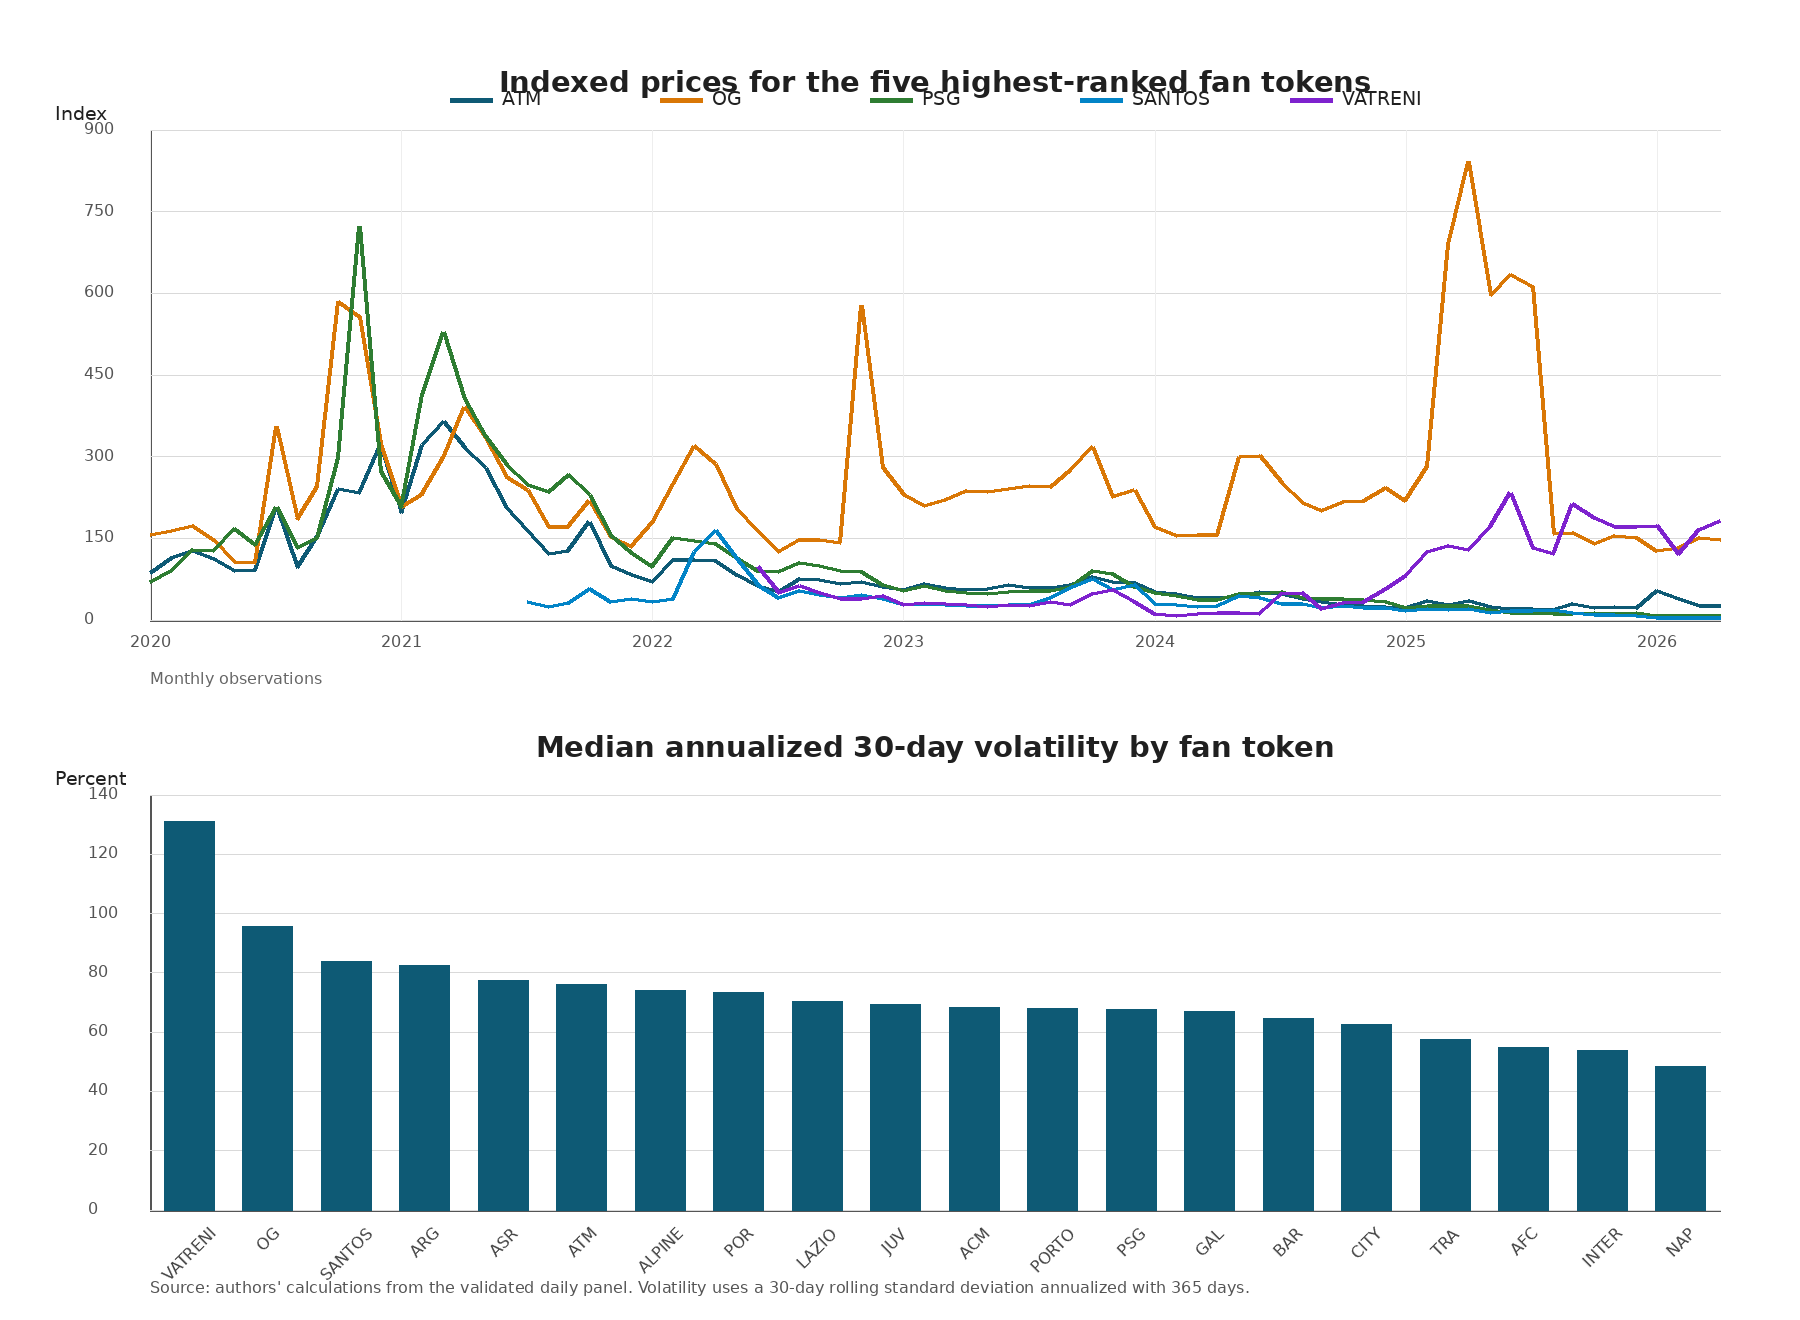
\includegraphics[width=\linewidth,height=.69\textheight,keepaspectratio]{figures/figure-1.png}
\captionof{figure}{Figure 1. Indexed monthly prices for the top five sample assets, alongside the median annualized 30-day volatility for all fan tokens.}
\end{minipage}\end{center}

The indexed-price panel shows repeated surges and reversals. It does not show a common monotonic path, so the series does not move in one direction together. Many prominent price peaks are seen in OG. PSG and ATM show sharp price increases during the early market expansion, while VATRENI shows increased volatility in a later time period. These price patterns can be seen in the chart, but are not formal statistical evidence. A large increase or decrease in prices, or a volatility spike are not enough to classify a bubble on their own. A right tailed unit root test needs to reject the null hypothesis, and the identified dates should be supported by planned validation methods in order to classify a bubble.

\subsection{5.6 Co-movement with the crypto market}

There is moderate co-movement in returns among the 190 token pairs. The pairwise correlation ranges from -0.01 to 0.849, with a mean of 0.392 and a median of 0.387. The majority of price fluctuation is unique to each token, as indicated by a correlation of around 0.39, or roughly 15\% shared return variation. Compared to Ethereum (0.338) or Bitcoin (0.314), fan tokens have a stronger correlation with Chiliz (0.421) and with each other (0.392). The cause of the remaining unshared variance cannot be explained by the correlation data. Although specific event and liquidity data are needed to validate this, club news and liquidity are plausible drivers of this independent movement.

\par\addvspace{5pt}\noindent\begin{minipage}{\linewidth}\reportcaption{Table 5. Distribution of token-level benchmark return correlations}

\begingroup\small\renewcommand{\arraystretch}{1.18}\setlength{\tabcolsep}{4pt}\arrayrulecolor{lightgray}
\noindent\begin{tabular}{|>{\raggedright\arraybackslash}p{0.242424\dimexpr\linewidth-10\tabcolsep-6\arrayrulewidth\relax}>{\raggedright\arraybackslash}p{0.189394\dimexpr\linewidth-10\tabcolsep-6\arrayrulewidth\relax}>{\raggedright\arraybackslash}p{0.189394\dimexpr\linewidth-10\tabcolsep-6\arrayrulewidth\relax}>{\raggedright\arraybackslash}p{0.189394\dimexpr\linewidth-10\tabcolsep-6\arrayrulewidth\relax}>{\raggedright\arraybackslash}p{0.189394\dimexpr\linewidth-10\tabcolsep-6\arrayrulewidth\relax}|}
\hline\rowcolor[HTML]{E8E8E8} \bfseries Benchmark & \bfseries Mean & \bfseries Median & \bfseries Minimum & \bfseries Maximum \\ \hline
Bitcoin & 0.314 & 0.316 & 0.119 & 0.406 \\ \hline
Chiliz & 0.421 & 0.421 & 0.114 & 0.556 \\ \hline
Ethereum & 0.338 & 0.345 & 0.091 & 0.440 \\ \hline
\end{tabular}\endgroup\end{minipage}\par\addvspace{5pt}

Three key design requirements for formal inference models are outlined in descriptive results. In addition to non-stationary volatility, models must take hefty tails into consideration. To properly evaluate severe market swings, cross-validation is essential. It is necessary to include token-specific methods into a pooled modeling framework. The existence of speculative bubbles is not confirmed by these first statistical findings alone.

The preceding methodology records the proposed design developed in Phase 2. The empirical analysis in Phase 3 uses the implemented settings reported below, including published reference thresholds, a 30-day dating rule, segmented return series and a local Bayesian ADF model. The proposed wild bootstrap, sequential KS-CPM validation and hierarchical predictor model should therefore be read as planned extensions rather than completed results. The June analysis and September extension retain their respective cutoffs.

\section{6 Empirical results}

\subsection{6.1 Results Overview}

\par\addvspace{5pt}\noindent\begin{minipage}{\linewidth}\reportcaption{Table 6. Summary of the June analysis and September extension}

\begingroup\small\renewcommand{\arraystretch}{1.18}\setlength{\tabcolsep}{4pt}\arrayrulecolor{lightgray}
\noindent\begin{tabular}{|>{\raggedright\arraybackslash}p{0.606061\dimexpr\linewidth-6\tabcolsep-4\arrayrulewidth\relax}>{\raggedright\arraybackslash}p{0.196970\dimexpr\linewidth-6\tabcolsep-4\arrayrulewidth\relax}>{\raggedright\arraybackslash}p{0.196970\dimexpr\linewidth-6\tabcolsep-4\arrayrulewidth\relax}|}
\hline\rowcolor[HTML]{E8E8E8} \bfseries Measure & \bfseries 30 June 2026 & \bfseries 19 September 2026 \\ \hline
Number of Fan Token observations & 37,662 & 39,282 \\ \hline
GSADF exceeded at 5 percent (Nominal) & 9 of 20 & 10 of 20 \\ \hline
Intervals of atleast 30 days for Fan Tokens & 0 & 2 \\ \hline
Number of changes detected across 23 assets (20 fan tokens + 3 reference) & 142 & 150 \\ \hline
Bayesian records in total (daily) & 45,672 & 47,535 \\ \hline
\end{tabular}\endgroup\end{minipage}\par\addvspace{5pt}

To understand and analyze if the findings change beyond the initial sample ending 30 June 2026, we extend the fan-token price data through September 2026 and add approximately 1620 observations. The September extension thus identified longer statistical intervals for Portugal and Argentina tokens where prices have been observed to fall by 69.9\% and 44.2\% respectively within these intervals. Such cases imply that a persistent statistical signal can accompany a severe market correction. It is imperative however that the economic interpretation of an episode or a statistical signal be accompanied by domain specific analysis of the "price path".

Volatility shifts are directly responsible for 76.8\% of the fan-token change points. The Bayesian model identified only five isolated days with strong local evidence. Such results can be explained with fan demand interacting with bursts of speculative interests, the matter of how long the demand lasts however matters as much as the size of the individual price movement. Unusual dynamics appeared across several tokens, but evidence for continuing speculative appreciation was much more limited.

\subsection{6.2 Study scope and data}

The study examines whether unusual fan-token price movements develop into persistent bubble episodes and how they relate to changes in market risk. The primary analysis runs through 30 June 2026 , the analysis also extends through 19 September 2026 to show how the findings change when the observation period is longer.

The sample includes 20 fan tokens and three benchmarks: Bitcoin, Ethereum and Chiliz. Fan-token price histories begin between 22 April 2020 and 27 November 2022. The June sample contains 37,662 valid fan-token price observations,ranging from 1,312 to 2,261 observations per token. Prices are daily USD closing prices organised by UTC calendar date. Daily returns are calculated as changes in natural-log prices multiplied by 100.

We used Archived Yahoo Finance histories and CoinGecko to procure the price data and the comparison between sample definition and sources respectively.

\subsection{6.3 Methods and decision rules}

The methods address three important yet related questions. Recursive ADF tests detect explosive price dynamics whereas BSADF dating measures how long those dynamics persist. Change-point and Bayesian models examine shifts in returns and local price behaviour. SADF holds the starting date fixed while GSADF tests alternative starting and ending dates mainly using regressions including an intercept and zero lagged differences and use the PSY minimum-window rule (Phillips, Shi, \& Yu, 2015).

\par\addvspace{5pt}\noindent\begin{minipage}{\linewidth}\reportcaption{Table 7. Implemented methods and decision rules}

\begingroup\small\renewcommand{\arraystretch}{1.18}\setlength{\tabcolsep}{4pt}\arrayrulecolor{lightgray}
\noindent\begin{tabular}{|>{\raggedright\arraybackslash}p{0.371212\dimexpr\linewidth-4\tabcolsep-3\arrayrulewidth\relax}>{\raggedright\arraybackslash}p{0.628788\dimexpr\linewidth-4\tabcolsep-3\arrayrulewidth\relax}|}
\hline\rowcolor[HTML]{E8E8E8} \bfseries Setting & \bfseries Value used \\ \hline
Recursive regression augmentation & Lagged differences (Zero difference) \\ \hline
Minimum regression window for fan tokens & PSY default rule resulting in 78 to 108 price observations \\ \hline
Reference thresholds & Published percentiles at 90\%, 95\% and 99\% \\ \hline
Dating rule & 30 consecutive days above the approximate endpoint threshold \\ \hline
Change point model & Separate standardized return mean and log squared return series \\ \hline
Segmentation rule & At least 30 observations per segment and a penalty of twice log sample size \\ \hline
Bayesian model & Local ADF slope with normal priors fixed standardized innovation variance and expected run length of 365 days \\ \hline
\end{tabular}\endgroup\end{minipage}\par\addvspace{5pt}

The analysis helps us understand and relate the statistical signals to their economic meanings asking three questions.

Does unusual price behaviour last long enough to resemble a continuing speculative process ?

Does such behaviour occur alongside repeated changes in trading conditions ?

How do explosive price dynamics relate to shifts in returns and local price behaviour?

\subsection{6.4 Recursive test results}

GSADF detected explosive signals in more tokens as compared to SADF. Nine of the 20 fan tokens exceed both the 5\% and 1\% GSADF reference thresholds. Four tokens (ATM , BAR , ASR and POR) exceed the 5 \% SADF reference threshold. GSADF tends to identify more signals because its flexible starting dates can isolate local episodes within a token's longer price history.

\par\addvspace{5pt}\noindent\begin{minipage}{\linewidth}\reportcaption{Table 8. Results through 30 June 2026}

\begingroup\small\renewcommand{\arraystretch}{1.18}\setlength{\tabcolsep}{4pt}\arrayrulecolor{lightgray}
\fontsize{9}{10.8}\selectfont
\noindent\begin{tabular}{|>{\raggedright\arraybackslash}p{0.128788\dimexpr\linewidth-14\tabcolsep-8\arrayrulewidth\relax}>{\raggedright\arraybackslash}p{0.101515\dimexpr\linewidth-14\tabcolsep-8\arrayrulewidth\relax}>{\raggedright\arraybackslash}p{0.109091\dimexpr\linewidth-14\tabcolsep-8\arrayrulewidth\relax}>{\raggedright\arraybackslash}p{0.113636\dimexpr\linewidth-14\tabcolsep-8\arrayrulewidth\relax}>{\raggedright\arraybackslash}p{0.174242\dimexpr\linewidth-14\tabcolsep-8\arrayrulewidth\relax}>{\raggedright\arraybackslash}p{0.178788\dimexpr\linewidth-14\tabcolsep-8\arrayrulewidth\relax}>{\raggedright\arraybackslash}p{0.193939\dimexpr\linewidth-14\tabcolsep-8\arrayrulewidth\relax}|}
\hline\rowcolor[HTML]{E8E8E8} \bfseries Token & \bfseries Prices & \bfseries SADF & \bfseries GSADF & \bfseries 95\% GSADF reference & \bfseries Exceeds reference & \bfseries Longest run days \\ \hline
VATRENI & 1,312 & -0.706 & 2.171 & 2.385 & No & 2 \\ \hline
OG & 2,201 & 0.929 & 6.025 & 2.463 & Yes & 9 \\ \hline
ATM & 2,201 & 3.097 & 5.028 & 2.463 & Yes & 7 \\ \hline
SANTOS & 1,673 & -1.144 & 2.195 & 2.416 & No & 2 \\ \hline
PSG & 2,211 & 0.584 & 4.106 & 2.463 & Yes & 10 \\ \hline
BAR & 2,198 & 2.485 & 3.913 & 2.462 & Yes & 14 \\ \hline
ASR & 2,201 & 2.738 & 4.582 & 2.463 & Yes & 7 \\ \hline
GAL & 2,214 & 0.609 & 4.674 & 2.464 & Yes & 11 \\ \hline
PORTO & 1,688 & -0.464 & 2.052 & 2.418 & No & 3 \\ \hline
CITY & 1,862 & -0.423 & 1.958 & 2.433 & No & 2 \\ \hline
LAZIO & 1,714 & -1.926 & 2.405 & 2.420 & No & 3 \\ \hline
JUV & 2,261 & -0.372 & 4.353 & 2.468 & Yes & 3 \\ \hline
ACM & 1,954 & -0.665 & 1.427 & 2.441 & No & 0 \\ \hline
AFC & 1,707 & 0.164 & 2.398 & 2.419 & No & 10 \\ \hline
ALPINE & 1,591 & -1.273 & 1.766 & 2.409 & No & 2 \\ \hline
INTER & 1,751 & 1.570 & 3.216 & 2.423 & Yes & 5 \\ \hline
TRA & 2,059 & -0.508 & 2.290 & 2.450 & No & 3 \\ \hline
ARG & 1,786 & -0.643 & 2.237 & 2.426 & No & 3 \\ \hline
NAP & 1,398 & 0.808 & 2.312 & 2.392 & No & 2 \\ \hline
POR & 1,680 & 2.660 & 3.847 & 2.417 & Yes & 22 \\ \hline
\end{tabular}\endgroup\end{minipage}\par\addvspace{5pt}

The table reports thresholds and persistence measures , The threshold column records the 95\% global GSADF reference values. The longest run metric counts the maximum number of consecutive days that the test statistic stays above the endpoint dating threshold, linking signal detection to persistence over time

OG and ATM have the largest GSADF statistics. OG records the highest statistic at 6.025, followed by ATM at 5.028. These results indicate explosive dynamics across several assets, consistent with bursts of speculative pressure in particular time windows. Whether that momentum persists and how economically significant it is depends on the dating results.

\subsection{6.5 Run lengths against BTC, ETH and CHZ}

None of the fan tokens reached a 30-day streak by 30 June 2026. Portugal's fan token came the closest with a 22-day streak from 5-26 August 2022, and another 16-day streak in late June 2026. The club tokens did not have long maximum streaks: Barcelona had a 14-day maximum, Galatasaray had 11 days, and both PSG and Arsenal had 10 days.

GSADF and the longest run metric are used to measure different things. GSADF identifies the strongest explosive episode seen in the data, while the dating metric captures persistence of upward momentum without interruptions. Nine tokens in the sample showed strong local explosive episodes, but none of them could maintain this momentum for 30 consecutive days.  

\par\addvspace{5pt}\noindent\begin{minipage}{\linewidth}\reportcaption{Table 9. Benchmark results through 30 June 2026}

\begingroup\small\renewcommand{\arraystretch}{1.18}\setlength{\tabcolsep}{4pt}\arrayrulecolor{lightgray}
\noindent\begin{tabular}{|>{\raggedright\arraybackslash}p{0.151515\dimexpr\linewidth-10\tabcolsep-6\arrayrulewidth\relax}>{\raggedright\arraybackslash}p{0.125758\dimexpr\linewidth-10\tabcolsep-6\arrayrulewidth\relax}>{\raggedright\arraybackslash}p{0.128788\dimexpr\linewidth-10\tabcolsep-6\arrayrulewidth\relax}>{\raggedright\arraybackslash}p{0.378788\dimexpr\linewidth-10\tabcolsep-6\arrayrulewidth\relax}>{\raggedright\arraybackslash}p{0.215152\dimexpr\linewidth-10\tabcolsep-6\arrayrulewidth\relax}|}
\hline\rowcolor[HTML]{E8E8E8} \bfseries Benchmark & \bfseries SADF & \bfseries GSADF & \bfseries Exceeds nominal 5\% GSADF threshold & \bfseries Longest run days \\ \hline
BTC & 2.290 & 3.889 & Yes & 27 \\ \hline
ETH & 1.712 & 2.228 & No & 10 \\ \hline
CHZ & 5.048 & 8.144 & Yes & 53 \\ \hline
\end{tabular}\endgroup\end{minipage}\par\addvspace{5pt}

Only Bitcoin and Chiliz exceed the 5\% GSADF threshold. Chiliz had a longest run of 53 days, from 2 March to 23 April 2021, and its BSADF statistic peaked at 8.144 on 12 March. Bitcoin’s longest run was 27 days, while Ethereum had 10 days. Using the same threshold, no fan token came close to Chiliz’s performance. These benchmarks show what a long lasting bubble episode looks like in this sample.

\subsubsection{6.5.1 Economic meaning of persistence}

A bubble can only persist if there is continuous demand to keep the prices rising. The short runs in fan tokens indicate that speculative interest rises sharply but then fades away quickly. Fans may hold the tokens due to their attachment or interest in the club, but speculative traders only care about being able to sell the token at a higher price later. The duration results suggest that fan demand and speculative demand rarely overlap for long enough to sustain an explosive price run.

\subsection{6.6 Changes in return behaviour}

Change-point analysis identifies 125 total shifts across the two fitted fan token series. Out of these 125, 29 consist of mean returns and other 96 are changes in log squared returns. Furthermore, 76.8\% of all the changes in the fan-token series were because of volatility changes. 17 other changes are introduced by benchmark assets. Therefore, we have 142 total changes across all 23 analyzed assets. Concludingly, variability in changing return is the primary source of the instability. 

\par\addvspace{6pt}\begin{center}\begin{minipage}{\linewidth}\centering
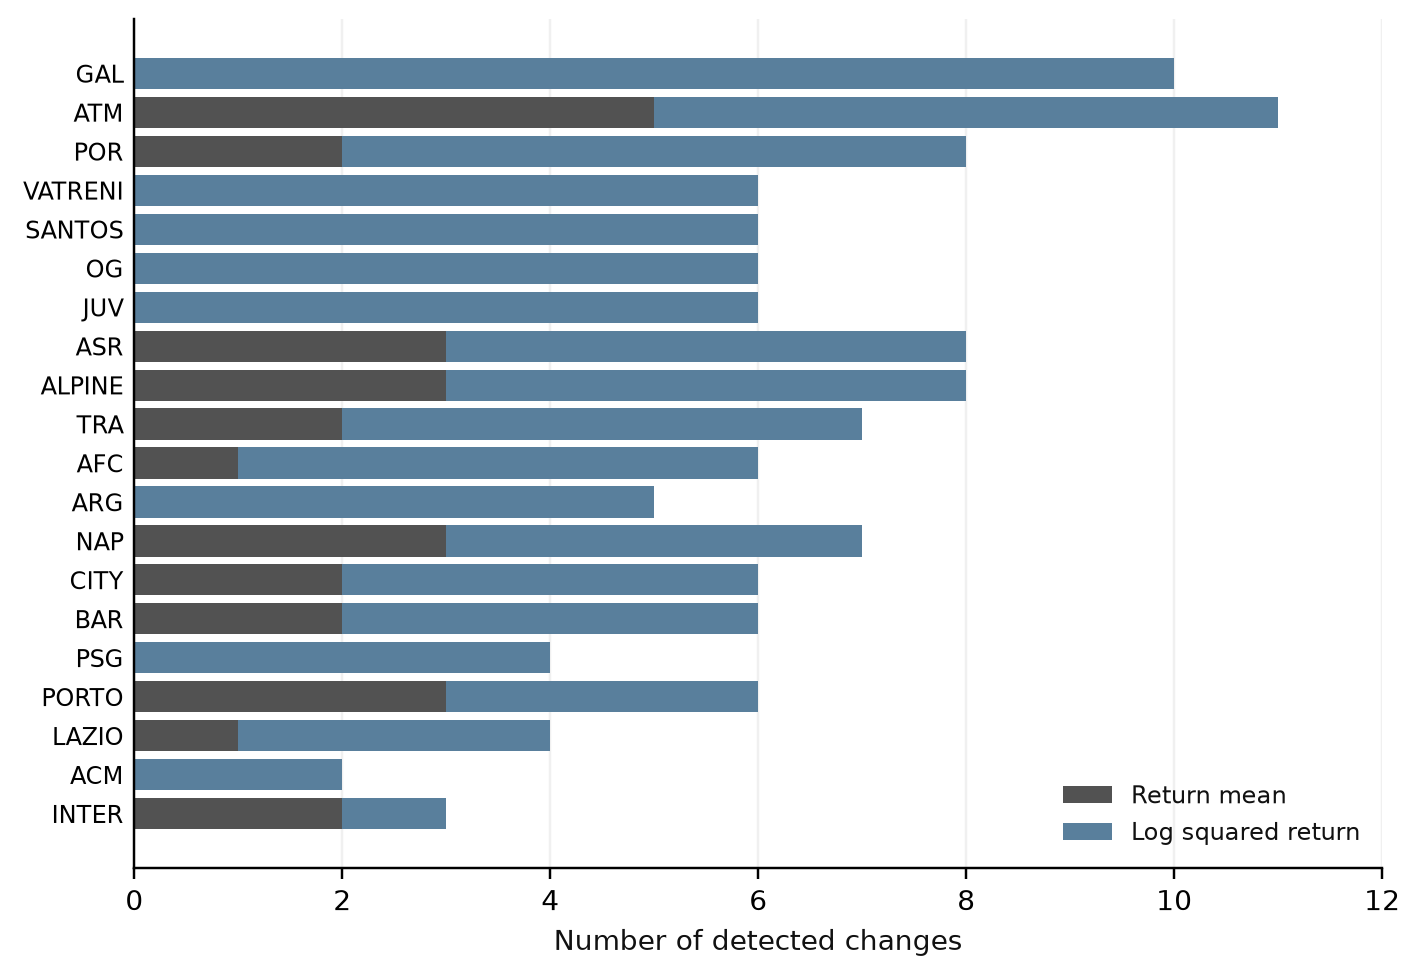
\includegraphics[width=\linewidth,height=.69\textheight,keepaspectratio]{figures/figure-2.png}
\captionof{figure}{Figure 2. Detected fan token changes through 30 June 2026 using a 30-day minimum segment and a penalty of twice log sample size}
\end{minipage}\end{center}

With 10 volatility changes, Galatasaray exhibits ten volatility changes which is the highest among fang tokens. Whereas, ATM shows five changes in mean returns. Additioanlly, 8 tokens have no shifts detected in mean returns. Token specific behaviour is importance for understanding the broader market as a token's volatility can change repeatedly with stable average returns. From an economic perspective, frequent volatility shift show differences in trading intensity and balance between actual fan demand and participation due to speculation. Market risk can increase due to unstable buying and selling. This does not require a prolonged upward price trend. These relationships explain why fan tokens experience turbulent trading without evidence of market bubbles.

\subsection{6.7 Bayesian evidence and agreement}

Across 37,642 daily estimates that were created by the Bayesian model, the median chance to find a positive local ADF slope was just 13.4 percent. In fact, only five daily observations (about 0.013 percent of the whole dataset) hit the 95 percent limit, and those show up on well sperated dates rather than a cluster. Looking at the day to day data we can observe occasional local acceleration instead of a sustained explosive regime.

\par\addvspace{5pt}\noindent\begin{minipage}{\linewidth}\reportcaption{Table 10. Isolated June sample posterior probabilities of at least 95 percent}

\begingroup\small\renewcommand{\arraystretch}{1.18}\setlength{\tabcolsep}{4pt}\arrayrulecolor{lightgray}
\noindent\begin{tabular}{|>{\raggedright\arraybackslash}p{0.151515\dimexpr\linewidth-8\tabcolsep-5\arrayrulewidth\relax}>{\raggedright\arraybackslash}p{0.242424\dimexpr\linewidth-8\tabcolsep-5\arrayrulewidth\relax}>{\raggedright\arraybackslash}p{0.303030\dimexpr\linewidth-8\tabcolsep-5\arrayrulewidth\relax}>{\raggedright\arraybackslash}p{0.303030\dimexpr\linewidth-8\tabcolsep-5\arrayrulewidth\relax}|}
\hline\rowcolor[HTML]{E8E8E8} \bfseries Token & \bfseries Date & \bfseries Positive slope probability percent & \bfseries New run probability percent \\ \hline
BAR & 2021-04-07 & 99.05 & 100.00 \\ \hline
GAL & 2021-05-14 & 98.61 & 11.50 \\ \hline
GAL & 2021-11-17 & 96.03 & 100.00 \\ \hline
ACM & 2021-02-24 & 98.84 & 0.27 \\ \hline
POR & 2024-03-11 & 95.47 & 100.00 \\ \hline
\end{tabular}\endgroup\end{minipage}\par\addvspace{5pt}

Those five high-probability observations belong to ACM, BAR, GAL, and POR. The BAR reading, the later GAL observation, and the POR one all line up perfectly with near-certain model resets, which points to some pretty abrupt shifts in the fitted local dynamics. Because of this, the table ends up clustering the strongest readings into just a handful of dates rather than any kind of sustained sequence.

\subsubsection{6.7.1 Reading the probability}

When a local ADF slope is positive, it tells us that price dynamics are favoring an explosive process within that fitted local regime. The model tracks the probability of this coefficient being positive, updating its assessment as new price history rolls in. And thanks to its run-length framework, the local relationship can just restart whenever conditions change. This follows the exact approach Adams and MacKay laid out in 2007.

If a speculative process was truly ongoing, you would expect to see support building across a sequence of dates as price pressure reinforces itself. Instead the high readings just pop up briefly and then fade away. That gives the Bayesian result a fairly intuitive economic meaning. It essentially shows that the strongest local disturbances don't stick around to become persistent features of the estimated price process.

When you read them together, the recursive and Bayesian results are really just describing the same broad persistence problem from different angles. The flexible GSADF search spots several strong episodes, but the daily Bayesian path doesn't show much continuing support for local explosiveness. Put that alongside the sheer predominance of volatility changes, and it all points to intermittent speculative pressure in markets where trading conditions are frequently shifting.

\subsection{6.8 Results from the September extension}

When we extend the data to 19 September 2026, there's an increase of 1620 fan-token prices and tokens above 5 percent GSADF reference rise from 9 to 10. ARG joins the group as well. Two runs now satisfy 30-day dating rule. Their price direction is central to the economic interpretation as this increased the persistence of statistical signals.

\par\addvspace{5pt}\noindent\begin{minipage}{\linewidth}\reportcaption{Table 11. Fan token intervals retained by the September run at the approximate 95 percent dating threshold}

\begingroup\small\renewcommand{\arraystretch}{1.18}\setlength{\tabcolsep}{4pt}\arrayrulecolor{lightgray}
\noindent\begin{tabular}{|>{\raggedright\arraybackslash}p{0.087879\dimexpr\linewidth-12\tabcolsep-7\arrayrulewidth\relax}>{\raggedright\arraybackslash}p{0.257576\dimexpr\linewidth-12\tabcolsep-7\arrayrulewidth\relax}>{\raggedright\arraybackslash}p{0.068182\dimexpr\linewidth-12\tabcolsep-7\arrayrulewidth\relax}>{\raggedright\arraybackslash}p{0.151515\dimexpr\linewidth-12\tabcolsep-7\arrayrulewidth\relax}>{\raggedright\arraybackslash}p{0.234848\dimexpr\linewidth-12\tabcolsep-7\arrayrulewidth\relax}>{\raggedright\arraybackslash}p{0.200000\dimexpr\linewidth-12\tabcolsep-7\arrayrulewidth\relax}|}
\hline\rowcolor[HTML]{E8E8E8} \bfseries Token & \bfseries Reference interval & \bfseries Days & \bfseries Price change percent & \bfseries Mean positive slope probability percent & \bfseries Endpoint status \\ \hline
ARG & 2026-07-21 to 2026-08-23 & 34 & -44.2 & 31.1 & Closed \\ \hline
POR & 2026-06-15 to 2026-09-19 & 97 & -69.9 & 40.5 & Ongoing at cutoff \\ \hline
\end{tabular}\endgroup\end{minipage}\par\addvspace{5pt}

Portugal has a 97-day interval which runs from 15 June to 19 September 2026 and Argentina has 34-day interval running from 21 July to 23 August. Portugal's interval remains open at the extension cutoff. Argentina's interval occur after the June assignment horizon entirely where as most part of Portugal's interval occur after the horizon. Primary sample could not yet observe the later developments that the extension captures.

\subsubsection{6.8.1 Economic interpretation of the price declines}

Portugal faces a price loss of 69.9 percent between the first and last closing prices of retained interval where as Argentina's loss is 44.2 percent. This clearly shows that these are intervals of pronounced downward repricing. An explosive-root signal has the property of unusual price dynamics and it can tend to stay high during a declining path. So this shows the economic character of both of these intervals is dominated by losses and correction.

Now, the average Bayesian positive-slope probability is 40.5 percent for Portugal and Argentina has 31.1 percent. Neither of them reaches the 95 percent mark on any day. A volatility change occurs on 1st August for Portugal. Combined effect links the unstable price adjustment to longer dating signals and contrastingly the daily model does not show enough support for the sustained local explosiveness.

The extension supports the central point of interpretation. Speculative interest can cause some unusual price behavior but a long statistic interval does not ensure the increase in price. The durability of demand decides if the momentum is continued or it gives way to a correction. These cases have the observed outcome as a major decline in token value.

\subsection{6.9 Price paths and the economic interpretation}

\par\addvspace{6pt}\begin{center}\begin{minipage}{\linewidth}\centering
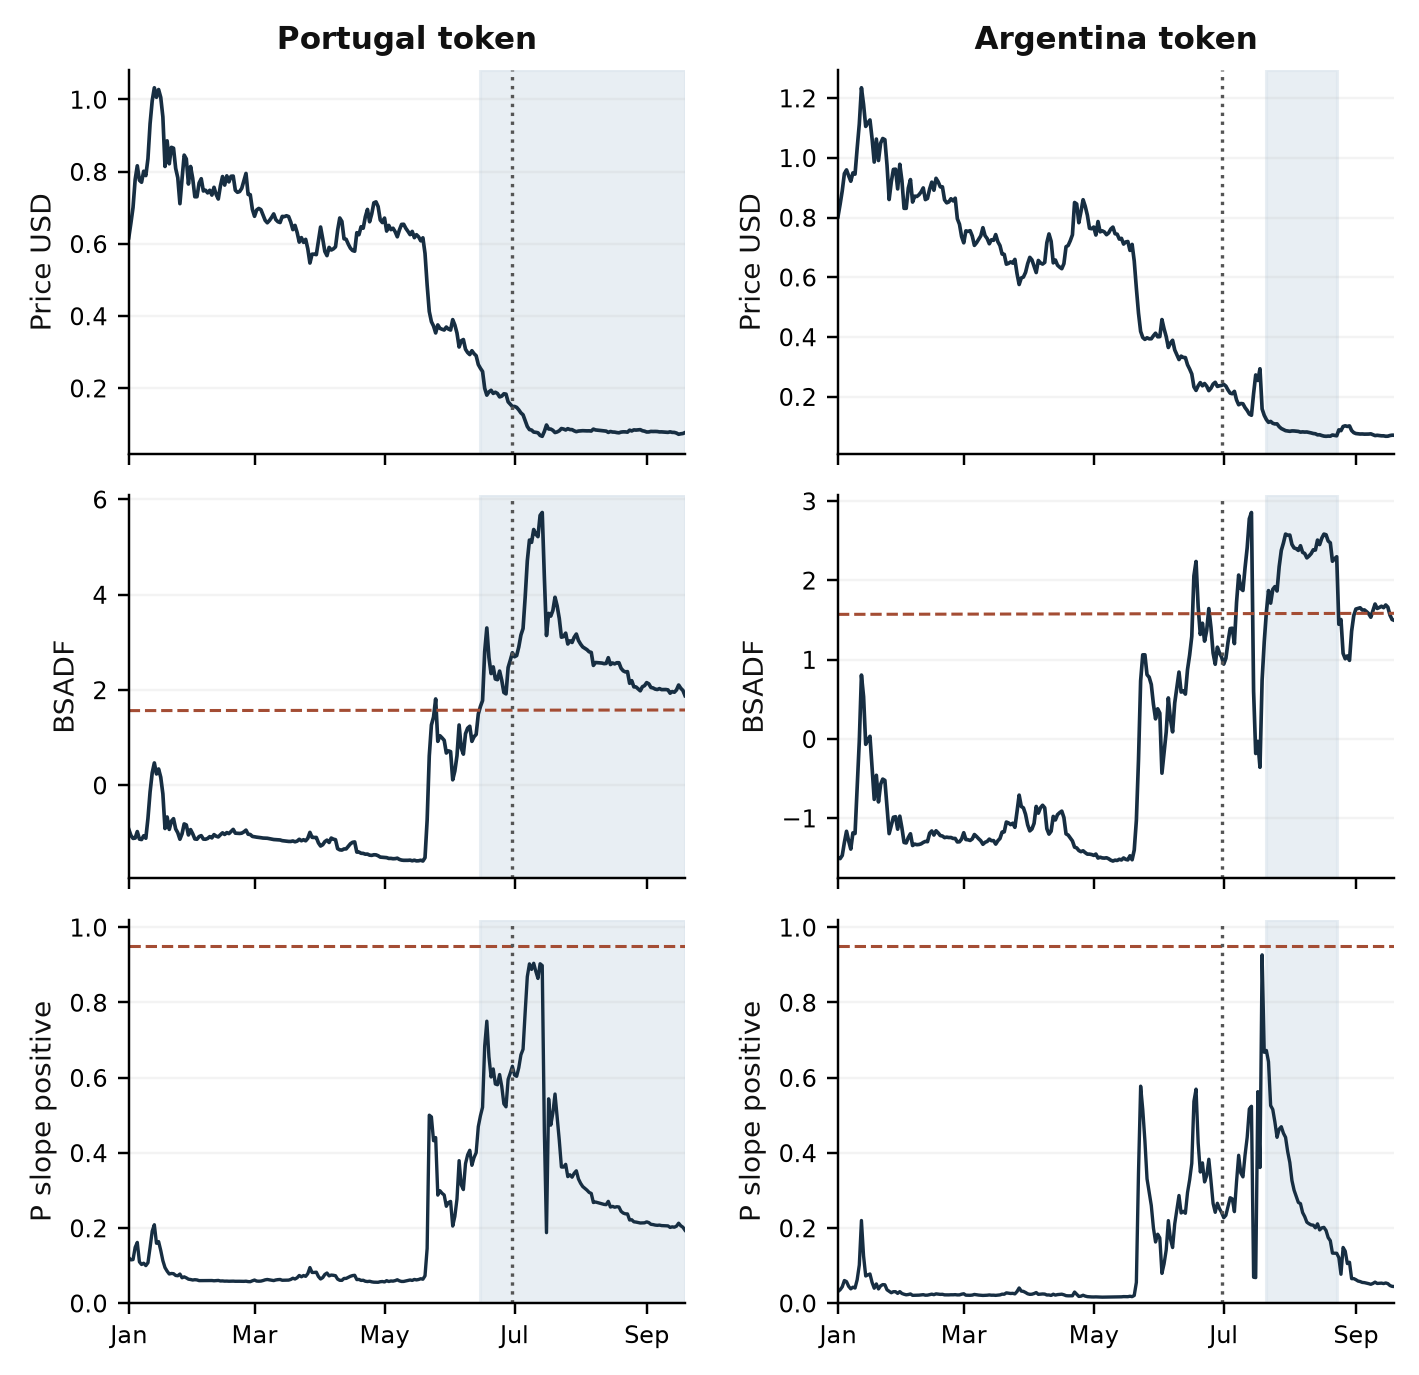
\includegraphics[width=\linewidth,height=.69\textheight,keepaspectratio]{figures/figure-3.png}
\captionof{figure}{Figure 3. September diagnostics for the two retained fan-token intervals. Shading marks the BSADF intervals. The vertical dotted line is 30 June 2026. Dashed lines show the reference dating threshold and the 95 percent Bayesian probability guide. Prices are USD closes.}
\end{minipage}\end{center}

Conditions across the shaded intervals show both of the price panels declining, whereas the dating statistic is still high. Bayesian paths also stay below the 95 percent mark. This concludes that the intervals show a forceful price adjustment within unusual statistical regimes. It also shows that persistence in an upward speculative process and persistence in a test signal are two different features of the data.

\section{7 Conclusion and study limitations}

\subsection{7.1 Conclusion}

Fan tokens exhibit explosive price dynamics in many cases. However, the evidence of persistent bubble episodes is limited. Out of the 20 fan tokens, 9 tokens exceed the GSADF reference by June. Even so, none of the 20 tokens satisfy the 30-day dating rule for a bubble episode. Volatility shifts account for more than 75\% of the identified change points in fan tokens. We only observe strong Bayesian readings on 5 isolated days. Therefore, the combined evidence puts intermittent explosiveness and changing market risk at the centre of the sample.

\subsection{7.2 Economic implications}

We observe a correlation between high speculative demand and increased fan attention, which is followed by momentum loss and repricing. Additionally, long statistical signals can overlap with other extreme price corrections. We see this in the September losses in Portugal and Argentina. Importantly, the primary issue is persistence. Unusual price paths are commonly observed across fan tokens, but the proof for prolonged speculative price surges remains low.

\subsection{7.3 Study limitations}

Test calibration and decision rules: Critical values in this analysis rely on interpolation or extrapolation from published tables, and endpoint dating utilizes an SADF-based approximation rather than a matched BSADF simulation. Statistical robustness could be improved through asset-specific calibration and a wild bootstrap under changing standard deviations. The counts and dates reported here ultimately reflect our specific chosen settings.

Bayesian specification: The model's probabilities depend on a local price coefficient and are calculated using fixed assumptions regarding variance, priors, and reset rules. Because full-sample scaling is used, these probabilities are inherently retrospective, capturing the ACM high reading right at initialization. Furthermore, since all methods analyze the exact same price data, methods complement rather than replicate each other.

Economic attribution and model scope: While price histories successfully track market risk and the persistence of price behaviors, isolating the direct impact of sporting events or attention-driven factors would require a separate event dataset. The current model does not attempt to explicitly classify the complete bubble life cycle. Futer research must include non-parametric validation and pooled predictor models.

Sample coverage and multiple comparisons: The fixed sample is based on a September snapshot, so applying it to the June analysis introduces potential selection bias and survivorship concerns. Additionally, without a multiplicity adjustment applied to the 20 global tests, the reported exceedances must be interpreted strictly as reference-threshold classifications for this specific group of tokens.

\clearpage
\section{Specific references}

\begin{reportreference}
[1] Assaf, A., Demir, E., \& Ersan, O. (2024). Detecting and date-stamping bubbles in fan tokens. International Review of Economics \& Finance, 92, 98-113. \url{https://doi.org/10.1016/j.iref.2024.01.039}
\end{reportreference}

\begin{reportreference}
[2] Boubaker, S., Liu, Z., Sui, T., \& Zhai, L. (2022). The mirror of history: How to statistically identify stock market bubble bursts. Journal of Economic Behavior \& Organization, 204, 128-147. \url{https://doi.org/10.1016/j.jebo.2022.09.024}
\end{reportreference}

\begin{reportreference}
[3] Harvey, D. I., Leybourne, S. J., Sollis, R., \& Taylor, A. M. R. (2016). Tests for explosive financial bubbles in the presence of non-stationary volatility. Journal of Empirical Finance, 38, 548-574. \url{https://doi.org/10.1016/j.jempfin.2015.09.002}
\end{reportreference}

\begin{reportreference}
[4] Harvey, D. I., Leybourne, S. J., Taylor, A. M. R., \& Zu, Y. (2025). A new heteroskedasticity-robust test for explosive bubbles. Journal of Time Series Analysis, 46(5), 846-866. \url{https://doi.org/10.1111/jtsa.12784}
\end{reportreference}

\begin{reportreference}
[5] Lui, Y. L., Phillips, P. C. B., \& Yu, J. (2024). Robust testing for explosive behavior with strongly dependent errors. Journal of Econometrics, 238(2), Article 105626. \url{https://doi.org/10.1016/j.jeconom.2023.105626}
\end{reportreference}

\begin{reportreference}
[6] Phillips, P. C. B., Wu, Y., \& Yu, J. (2011). Explosive behavior in the 1990s Nasdaq: When did exuberance escalate asset values? International Economic Review, 52(1), 201-226. \url{https://doi.org/10.1111/j.1468-2354.2010.00625.x}
\end{reportreference}

\begin{reportreference}
[7] Phillips, P. C. B., Shi, S., \& Yu, J. (2015a). Testing for multiple bubbles: Historical episodes of exuberance and collapse in the S\&P 500. International Economic Review, 56(4), 1043-1078. \url{https://doi.org/10.1111/iere.12132}
\end{reportreference}

\begin{reportreference}
[8] Phillips, P. C. B., Shi, S., \& Yu, J. (2015b). Testing for multiple bubbles: Limit theory of real-time detectors. International Economic Review, 56(4), 1079-1134. \url{https://doi.org/10.1111/iere.12131}
\end{reportreference}

\begin{reportreference}
[9] Ross, G. J., \& Adams, N. M. (2012). Two nonparametric control charts for detecting arbitrary distribution changes. Journal of Quality Technology, 44(2), 102-116.
\end{reportreference}

\begin{reportreference}
[10] Thies, S., \& Molnár, P. (2018). Bayesian change point analysis of Bitcoin returns. Finance Research Letters, 27, 223-227. \url{https://doi.org/10.1016/j.frl.2018.03.018}
\end{reportreference}

\begin{reportreference}
[11] Vidal-Tomás, D. (2024). Blockchain, sport and fan tokens. Journal of Economic Studies, 51(1), 24-38. \url{https://doi.org/10.1108/JES-02-2023-0094}
\end{reportreference}

\begin{reportreference}
[12] Vriz, G. L., \& Grossi, L. (2026). Green bubbles: A four-stage paradigm for detection and propagation. Energy Economics, 154, Article 109095. \url{https://doi.org/10.1016/j.eneco.2025.109095}
\end{reportreference}

\clearpage
\section{References}

\begin{reportreference}
Agnese, P., \& Xiao, Y. (2025). Tokenization in soccer leagues. Is fan engagement for real? Research in International Business and Finance, 76, 102827. \url{https://doi.org/10.1016/j.ribaf.2025.102827}
\end{reportreference}

\begin{reportreference}
Ante, L., Schellinger, B., \& Wazinski, F.-P. (2023). Enhancing trust, efficiency, and empowerment in sports: Developing a blockchain-based fan token framework. ECIS 2023 Research Papers (Paper 234). \url{https://aisel.aisnet.org/ecis2023_rp/234}
\end{reportreference}

\begin{reportreference}
Ante, L., Saggu, A., Schellinger, B., \& Wazinski, F.-P. (2024a). Voting participation and engagement in blockchain-based fan tokens. Electronic Markets, 34, Article 26. \url{https://doi.org/10.1007/s12525-024-00709-z}
\end{reportreference}

\begin{reportreference}
Ante, L., Schellinger, B., \& Demir, E. (2024b). The impact of football games and sporting performance on intra-day fan token returns. Journal of Business Economics, 94(5), 813-850. \url{https://doi.org/10.1007/s11573-023-01187-z}
\end{reportreference}

\begin{reportreference}
Ante, L., Henninger, L., Bauers, S. B., \& Schellinger, B. (2025). Blockchain-based fan tokens as a strategic resource for sports clubs: Opportunities, challenges, and a stakeholder-oriented model. Digital Business, 5(2), 100137. \url{https://doi.org/10.1016/j.digbus.2025.100137}
\end{reportreference}

\begin{reportreference}
Assaf, A., Demir, E., \& Ersan, O. (2024). Detecting and date-stamping bubbles in fan tokens. International Review of Economics \& Finance, 92, 98-113. \url{https://doi.org/10.1016/j.iref.2024.01.039}
\end{reportreference}

\begin{reportreference}
Bai, J., \& Perron, P. (1998). Estimating and testing linear models with multiple structural changes. Econometrica, 66(1), 47-78. \url{https://doi.org/10.2307/2998540}
\end{reportreference}

\begin{reportreference}
Bai, J., \& Perron, P. (2003). Computation and analysis of multiple structural change models. Journal of Applied Econometrics, 18(1), 1-22. \url{https://doi.org/10.1002/jae.659}
\end{reportreference}

\begin{reportreference}
Ben Yaala, S., \& Henchiri, J. E. (2025). Detecting and analyzing explosive bubbles and their relationship with volatility: Evidence from Tunisia. RAUSP Management Journal, 60(1), 86-101. \url{https://doi.org/10.1108/RAUSP-05-2024-0097}
\end{reportreference}

\begin{reportreference}
Blom, M. J., \& Henriques Pereira, M. (2026). Do match surprises move fan token prices? Evidence from UEFA competitions. Finance Research Letters, 90, 109349. \url{https://doi.org/10.1016/j.frl.2025.109349}
\end{reportreference}

\begin{reportreference}
Boubaker, S., Liu, Z., Sui, T., \& Zhai, L. (2022). The mirror of history: How to statistically identify stock market bubble bursts. Journal of Economic Behavior \& Organization, 204, 128-147. \url{https://doi.org/10.1016/j.jebo.2022.09.024}
\end{reportreference}

\begin{reportreference}
Cong, L. W., Li, Y., \& Wang, N. (2021). Tokenomics: Dynamic adoption and valuation. The Review of Financial Studies, 34(3), 1105-1155. \url{https://doi.org/10.1093/rfs/hhaa089}
\end{reportreference}

\begin{reportreference}
Demir, E., Ersan, O., \& Popesko, B. (2022). Are fan tokens fan tokens? Finance Research Letters, 47, 102736. \url{https://doi.org/10.1016/j.frl.2022.102736}
\end{reportreference}

\begin{reportreference}
Diniz, R., de Prince, D., \& Maciel, L. (2023). Bubble detection in Bitcoin and Ethereum and its relationship with volatility regimes. Journal of Economic Studies, 50(3), 429-447. \url{https://doi.org/10.1108/JES-09-2021-0452}
\end{reportreference}

\begin{reportreference}
Enoksen, F. A., Landsnes, C. J., Lučivjanská, K., \& Molnár, P. (2020). Understanding risk of bubbles in cryptocurrencies. Journal of Economic Behavior \& Organization, 176, 129-144. \url{https://doi.org/10.1016/j.jebo.2020.05.005}
\end{reportreference}

\begin{reportreference}
Filimonov, V., \& Sornette, D. (2013). A stable and robust calibration scheme of the log-periodic power law model. Physica A: Statistical Mechanics and its Applications, 392(17), 3698-3707. \url{https://doi.org/10.1016/j.physa.2013.04.012}
\end{reportreference}

\begin{reportreference}
Harvey, D. I., Leybourne, S. J., Sollis, R., \& Taylor, A. M. R. (2016). Tests for explosive financial bubbles in the presence of non-stationary volatility. Journal of Empirical Finance, 38, 548-574. \url{https://doi.org/10.1016/j.jempfin.2015.09.002}
\end{reportreference}

\begin{reportreference}
Harvey, D. I., Leybourne, S. J., Taylor, A. M. R., \& Zu, Y. (2025). A new heteroskedasticity-robust test for explosive bubbles. Journal of Time Series Analysis, 46(5), 846-866. \url{https://doi.org/10.1111/jtsa.12784}
\end{reportreference}

\begin{reportreference}
Haykir, O., \& Yagli, I. (2022). Speculative bubbles and herding in cryptocurrencies. Financial Innovation, 8, Article 78. \url{https://doi.org/10.1186/s40854-022-00383-0}
\end{reportreference}

\begin{reportreference}
Kaur, M., Jain, J., \& Sood, K. (2024). 'All are investing in crypto, I fear of being missed out': Examining the influence of herding, loss aversion, and overconfidence in the cryptocurrency market with the mediating effect of FOMO. Quality \& Quantity, 58(3), 2237-2263. \url{https://doi.org/10.1007/s11135-023-01739-z}
\end{reportreference}

\begin{reportreference}
Killick, R., Fearnhead, P., \& Eckley, I. A. (2012). Optimal detection of changepoints with a linear computational cost. Journal of the American Statistical Association, 107(500), 1590-1598. \url{https://doi.org/10.1080/01621459.2012.737745}
\end{reportreference}

\begin{reportreference}
Kindleberger, C. P. (1978). Manias, panics, and crashes: A history of financial crises. Basic Books.
\end{reportreference}

\begin{reportreference}
Kindleberger, C. P., \& Aliber, R. Z. (2005). Manias, panics, and crashes: A history of financial crises (5th ed.). John Wiley \& Sons.
\end{reportreference}

\begin{reportreference}
Lopez-Gonzalez, H., \& Griffiths, M. D. (2023). Gambling-like features in fan tokens. Journal of Gambling Studies, 39, 1579-1596. \url{https://doi.org/10.1007/s10899-023-10215-0}
\end{reportreference}

\begin{reportreference}
Lui, Y. L., Phillips, P. C. B., \& Yu, J. (2024). Robust testing for explosive behavior with strongly dependent errors. Journal of Econometrics, 238(2), 105626. \url{https://doi.org/10.1016/j.jeconom.2023.105626}
\end{reportreference}

\begin{reportreference}
Luo, X., Kihulgoda, D., Patrick-Bienwi, M., Olufunso-Ajibike, A., Akpobasa, T., \& Abbile, T. (2026). From the pitch to the market: What determines fan token prices dynamics and trading activities? Cogent Social Sciences, 12(1), 2631196. \url{https://doi.org/10.1080/23311886.2026.2631196}
\end{reportreference}

\begin{reportreference}
Phillips, P. C. B., Shi, S., \& Yu, J. (2015a). Testing for multiple bubbles: Historical episodes of exuberance and collapse in the S\&P 500. International Economic Review, 56(4), 1043-1078. \url{https://doi.org/10.1111/iere.12132}
\end{reportreference}

\begin{reportreference}
Phillips, P. C. B., Shi, S., \& Yu, J. (2015b). Testing for multiple bubbles: Limit theory of real-time detectors. International Economic Review, 56(4), 1079-1134. \url{https://doi.org/10.1111/iere.12131}
\end{reportreference}

\begin{reportreference}
Phillips, P. C. B., Wu, Y., \& Yu, J. (2011). Explosive behavior in the 1990s Nasdaq: When did exuberance escalate asset values? International Economic Review, 52(1), 201-226. \url{https://doi.org/10.1111/j.1468-2354.2010.00625.x}
\end{reportreference}

\begin{reportreference}
Ross, G. J., \& Adams, N. M. (2012). Two nonparametric control charts for detecting arbitrary distribution changes. Journal of Quality Technology, 44(2), 102-116. \url{https://doi.org/10.1080/00224065.2012.11917887}
\end{reportreference}

\begin{reportreference}
Saggu, A., Ante, L., \& Demir, E. (2024). Anticipatory gains and event-driven losses in blockchain-based fan tokens: Evidence from the FIFA World Cup. Research in International Business and Finance, 70, 102333. \url{https://doi.org/10.1016/j.ribaf.2024.102333}
\end{reportreference}

\begin{reportreference}
Scharnowski, M., Scharnowski, S., \& Zimmermann, L. (2023). Fan tokens: Sports and speculation on the blockchain. Journal of International Financial Markets, Institutions and Money, 89, 101880. \url{https://doi.org/10.1016/j.intfin.2023.101880}
\end{reportreference}

\begin{reportreference}
Shahzad, S. J. H., Anas, M., \& Bouri, E. (2022). Price explosiveness in cryptocurrencies and Elon Musk's tweets. Finance Research Letters, 44, 102695. \url{https://doi.org/10.1016/j.frl.2022.102695}
\end{reportreference}

\begin{reportreference}
Thies, S., \& Molnár, P. (2018). Bayesian change point analysis of Bitcoin returns. Finance Research Letters, 27, 223-227. \url{https://doi.org/10.1016/j.frl.2018.03.018}
\end{reportreference}

\begin{reportreference}
Vidal-Tomás, D. (2024). Blockchain, sport and fan tokens. Journal of Economic Studies, 51(1), 24-38. \url{https://doi.org/10.1108/JES-02-2023-0094}
\end{reportreference}

\begin{reportreference}
Vriz, G. L., \& Grossi, L. (2026). Green bubbles: A four-stage paradigm for detection and propagation. Energy Economics, 154, 109095. \url{https://doi.org/10.1016/j.eneco.2025.109095}
\end{reportreference}

\section{Data sources}

\begin{reportreference}
[1] CoinGecko. Fan-token category market snapshot and historical market-chart endpoints. \url{https://www.coingecko.com/en/categories/fan-token}
\end{reportreference}

\begin{reportreference}
[2] Yahoo Finance. Daily chart service for historical OHLC prices and reported volume. \url{https://finance.yahoo.com/}
\end{reportreference}

\begin{reportreference}
[3] Binance. Spot-market daily klines and official listing announcements used to validate flagged observations. \url{https://www.binance.com/}
\end{reportreference}

\begin{reportreference}
[4] CoinGlass. OG historical market data used to corroborate the 23 December 2020 price move. \url{https://www.coinglass.com/currencies/OG/historical-data}
\end{reportreference}

\clearpage
\section{Appendix A Supplementary Figures and Diagnostic Results}
{\small Source: archived project data and results.\par}
\subsection{A.1 Price and volatility}
\noindent\begin{minipage}{\linewidth}\centering
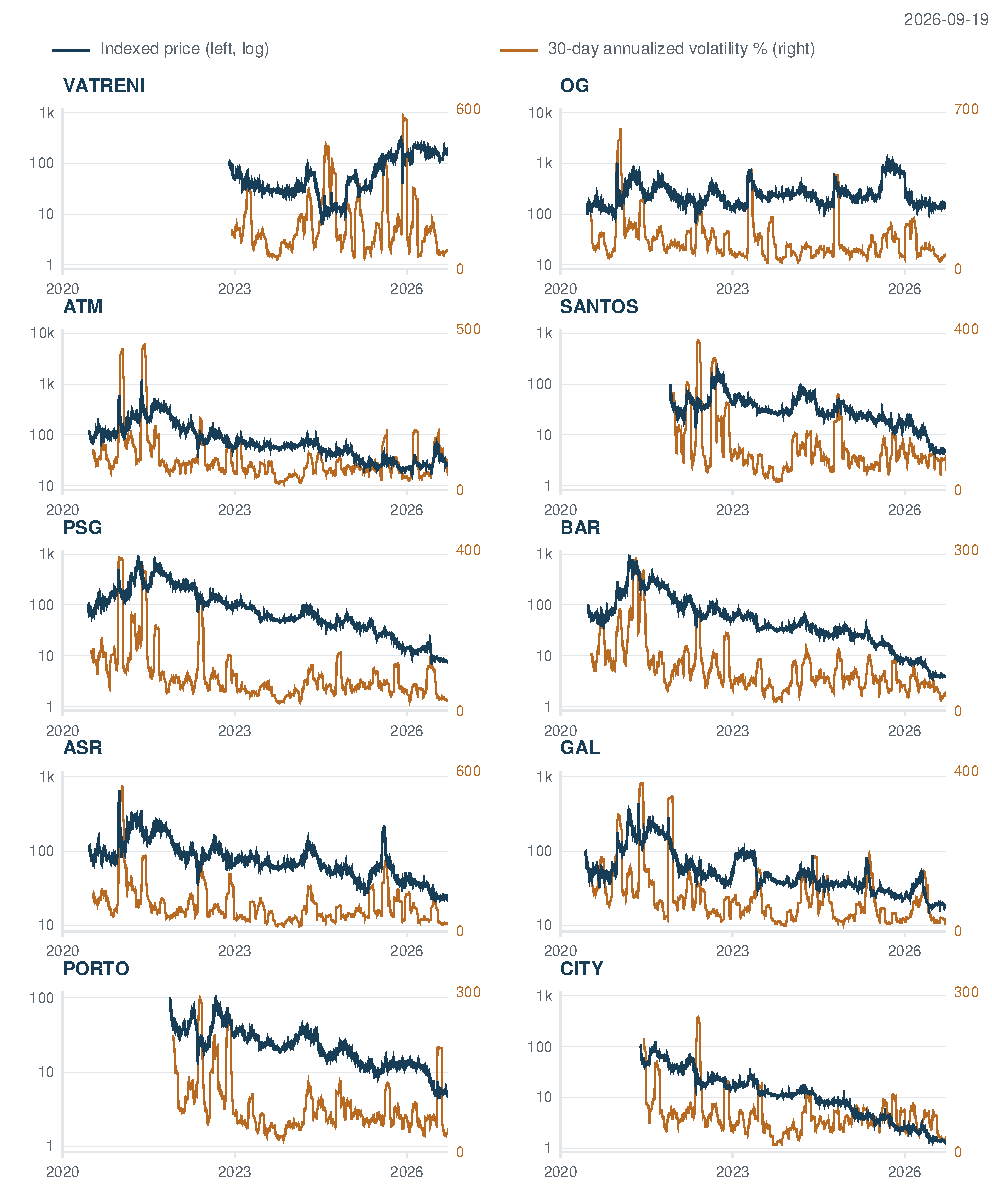
\includegraphics[width=\linewidth,height=.80\textheight,keepaspectratio]{figures/appendix/figure-A1.pdf}
\captionof{figure}{Figure A.1 Token profiles 1-10.}
\end{minipage}
\clearpage
\noindent\begin{minipage}{\linewidth}\centering
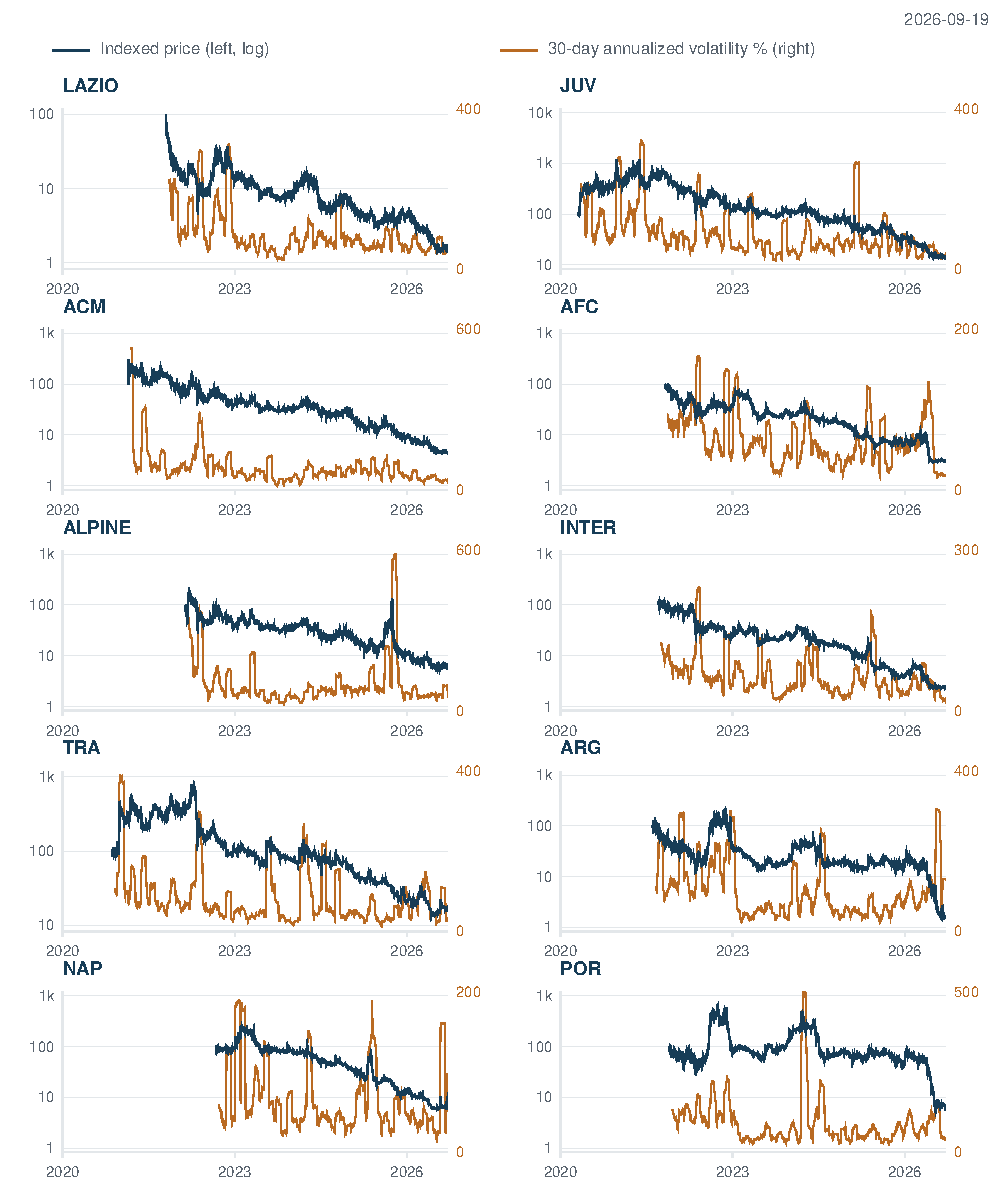
\includegraphics[width=\linewidth,height=.80\textheight,keepaspectratio]{figures/appendix/figure-A2.pdf}
\captionof{figure}{Figure A.2 Token profiles 11-20.}
\end{minipage}
\clearpage
\subsection{A.2 BSADF diagnostics}
\noindent\begin{minipage}{\linewidth}\centering
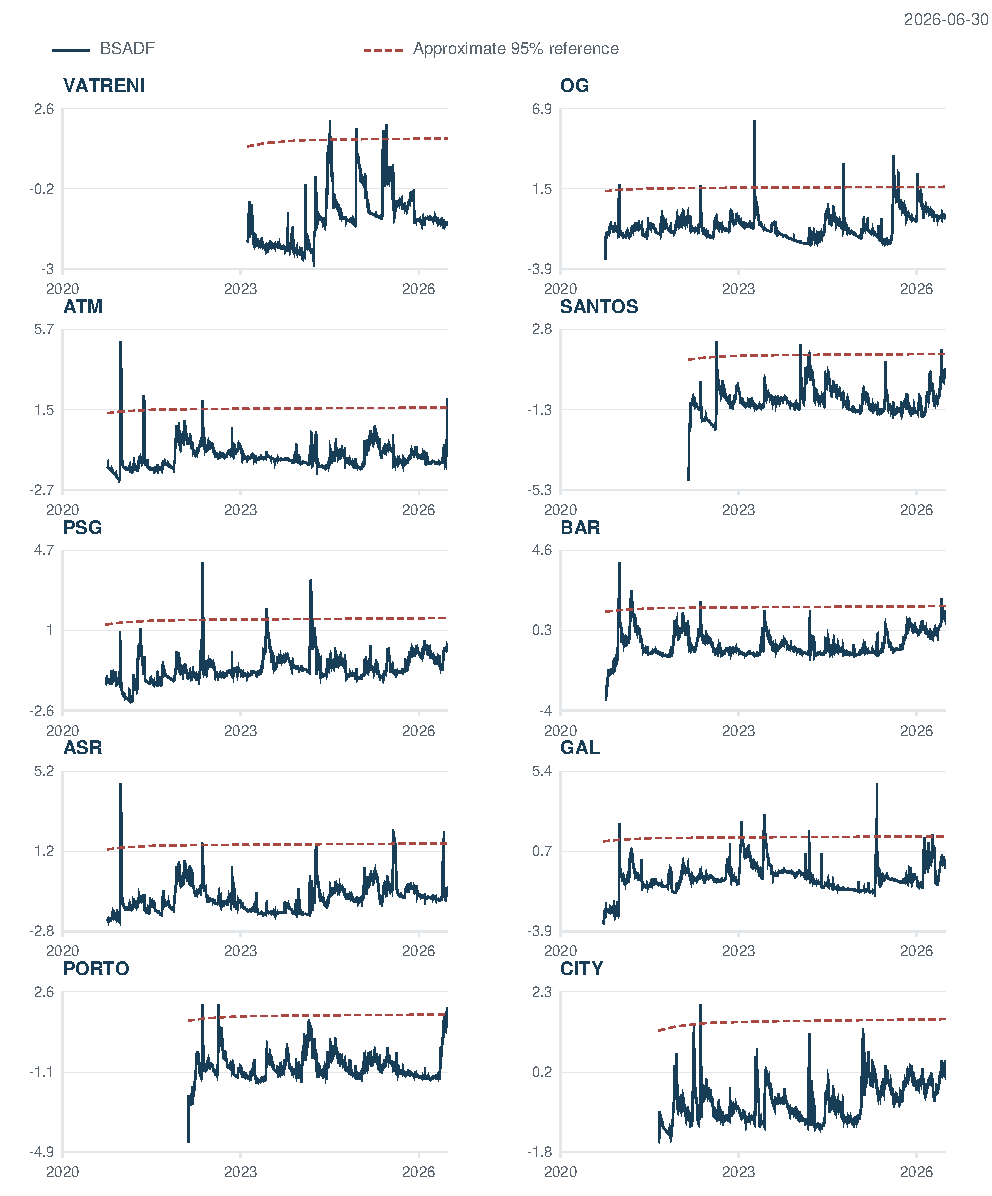
\includegraphics[width=\linewidth,height=.80\textheight,keepaspectratio]{figures/appendix/figure-A3.pdf}
\captionof{figure}{Figure A.3 BSADF paths 1-10.}
\end{minipage}
\clearpage
\noindent\begin{minipage}{\linewidth}\centering
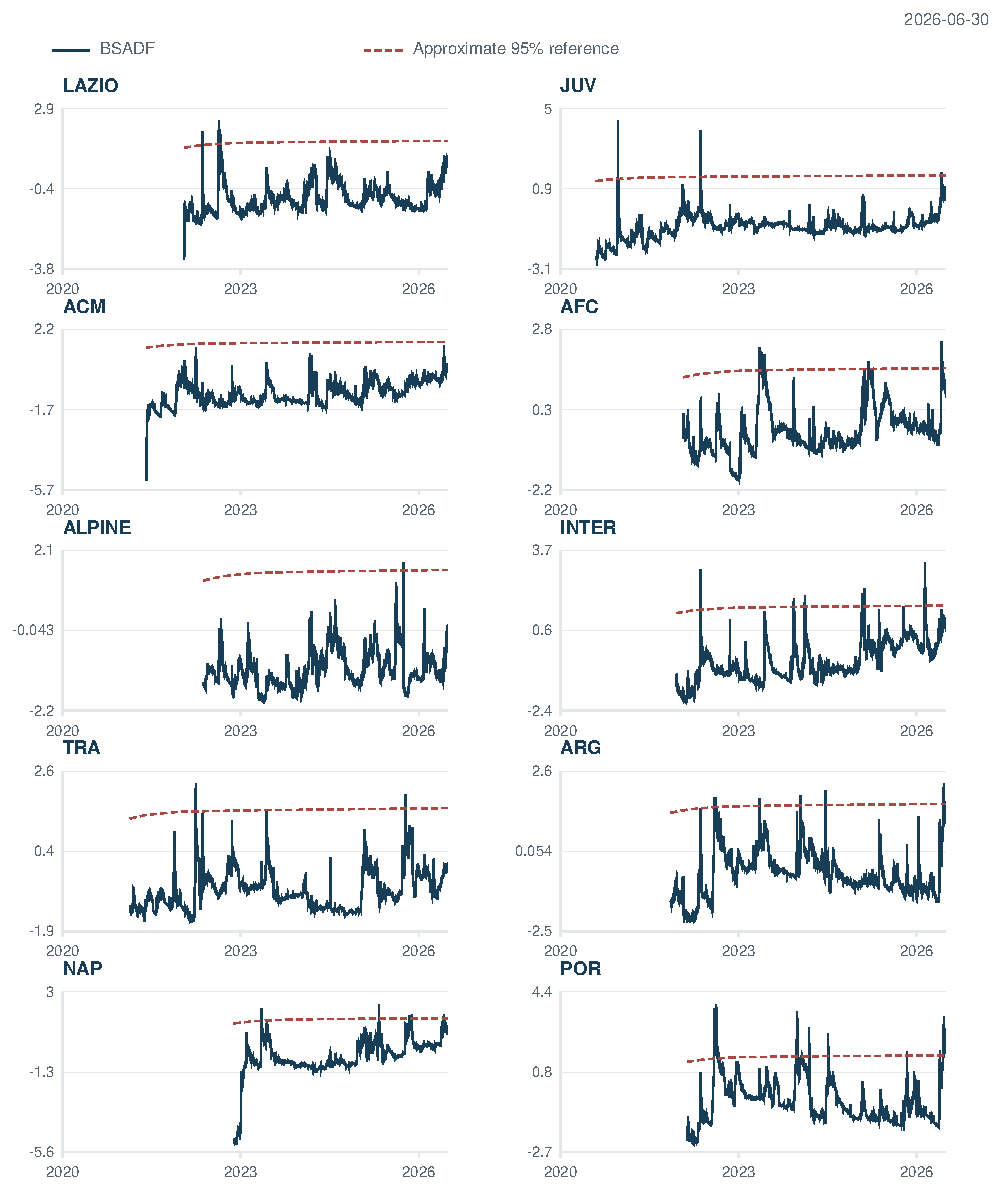
\includegraphics[width=\linewidth,height=.80\textheight,keepaspectratio]{figures/appendix/figure-A4.pdf}
\captionof{figure}{Figure A.4 BSADF paths 11-20.}
\end{minipage}
\clearpage
\subsection{A.3 Return change points}
\noindent\begin{minipage}{\linewidth}\centering
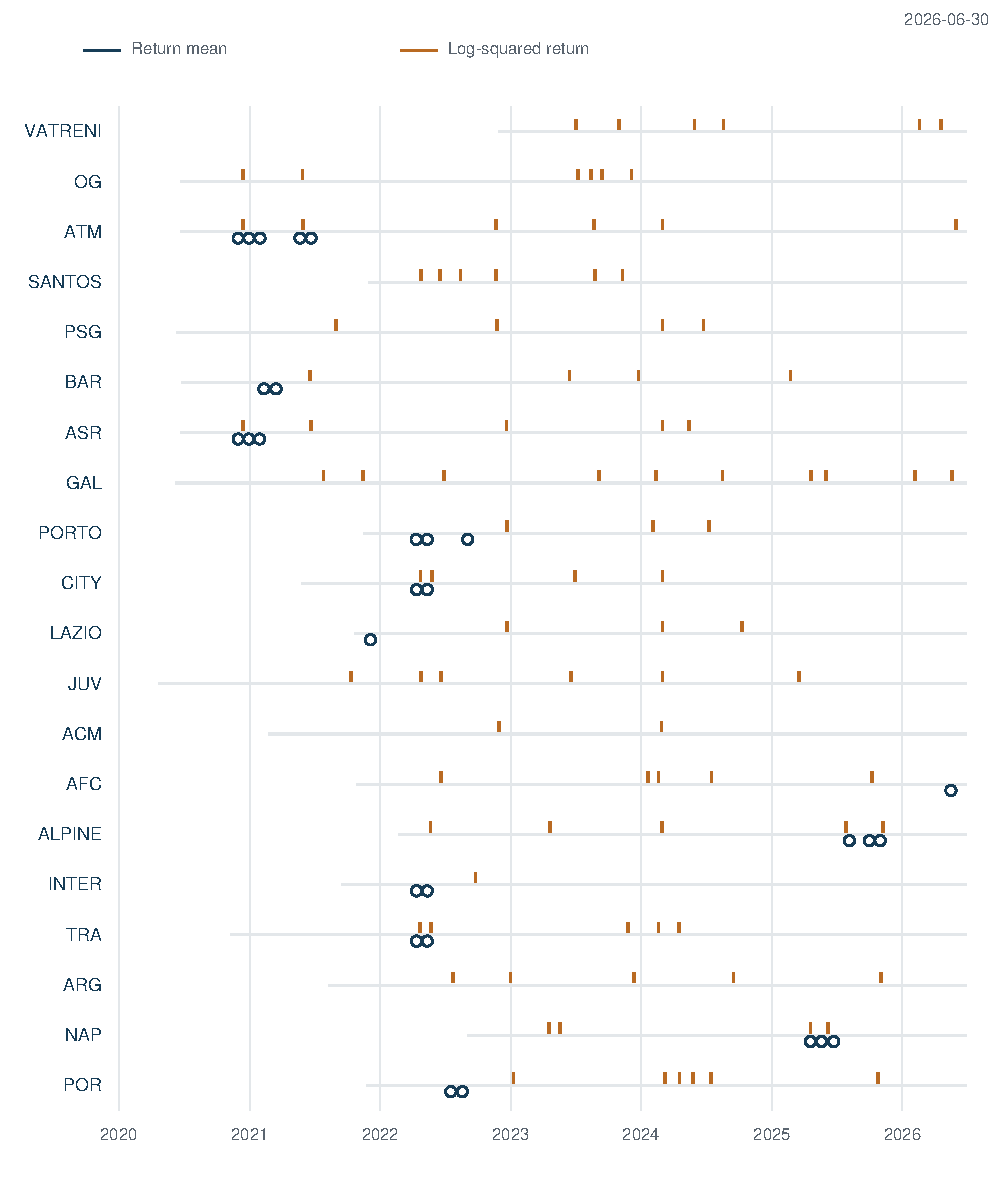
\includegraphics[width=\linewidth,height=.80\textheight,keepaspectratio]{figures/appendix/figure-A5.pdf}
\captionof{figure}{Figure A.5 Change-point dates.}
\end{minipage}
\clearpage
\subsection{A.4 Bayesian probabilities}
\noindent\begin{minipage}{\linewidth}\centering
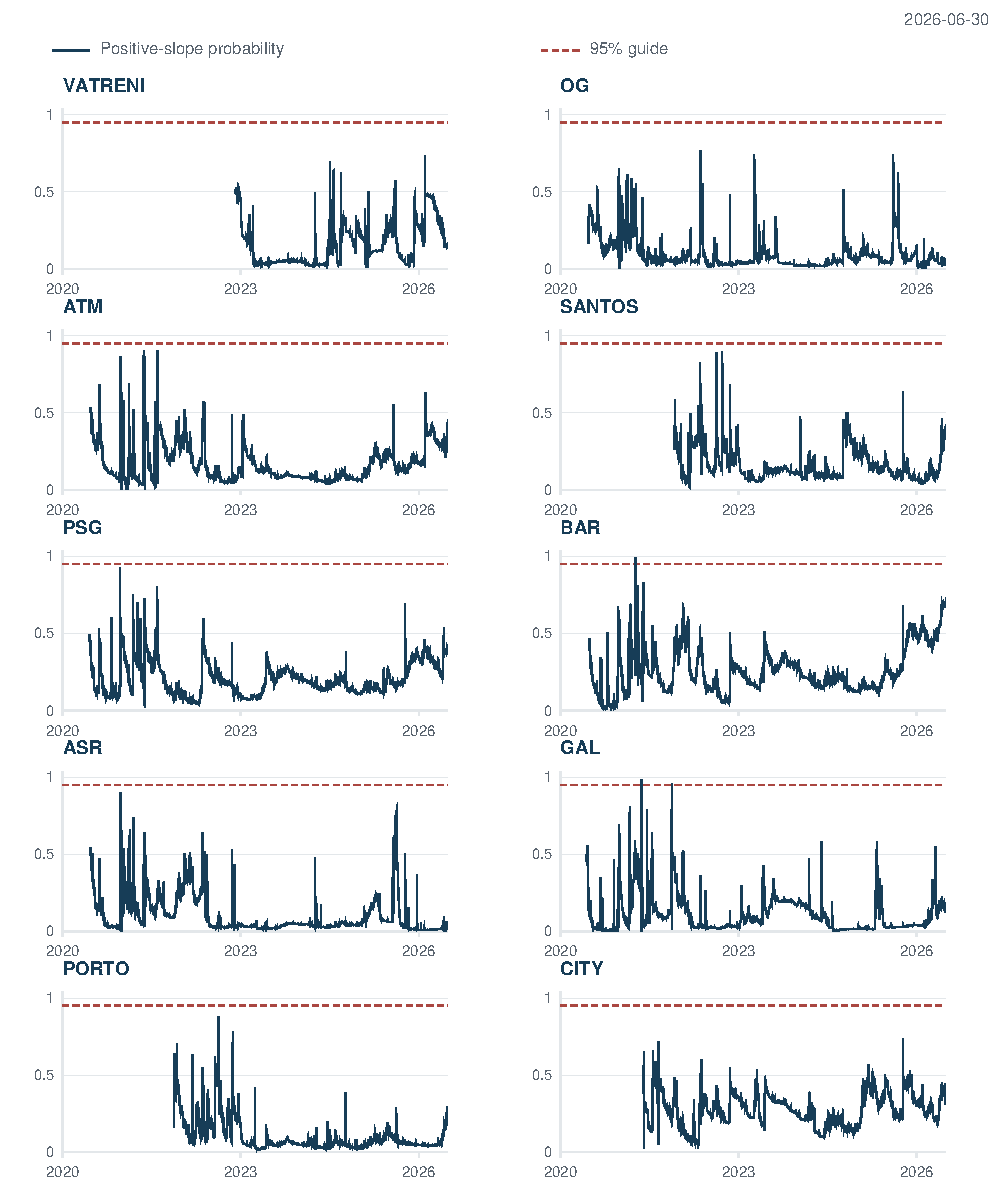
\includegraphics[width=\linewidth,height=.80\textheight,keepaspectratio]{figures/appendix/figure-A6.pdf}
\captionof{figure}{Figure A.6 Bayesian paths 1-10.}
\end{minipage}
\clearpage
\noindent\begin{minipage}{\linewidth}\centering
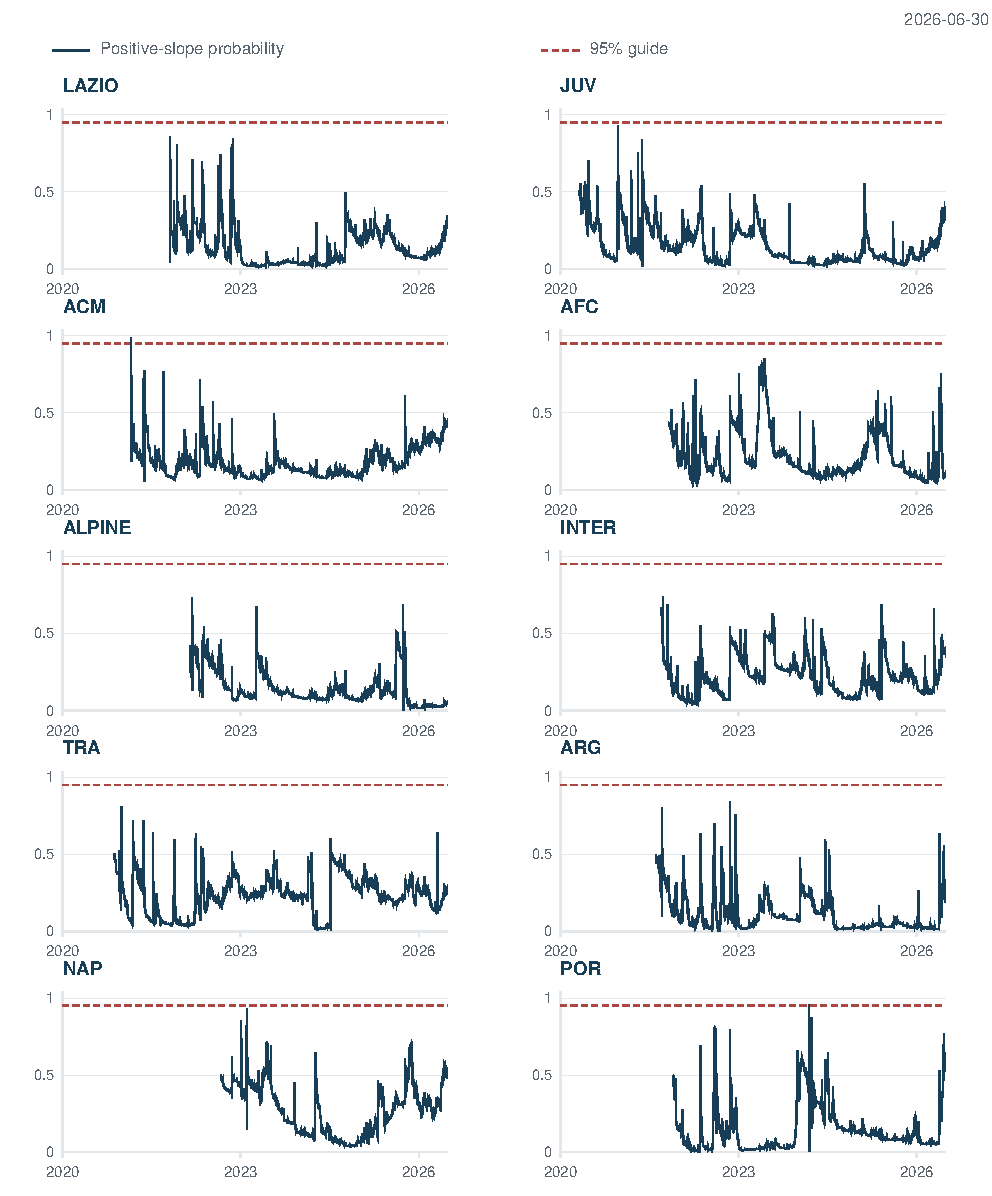
\includegraphics[width=\linewidth,height=.80\textheight,keepaspectratio]{figures/appendix/figure-A7.pdf}
\captionof{figure}{Figure A.7 Bayesian paths 11-20.}
\end{minipage}
\clearpage
\subsection{A.5 Benchmark comparisons}
\noindent\begin{minipage}{\linewidth}\centering
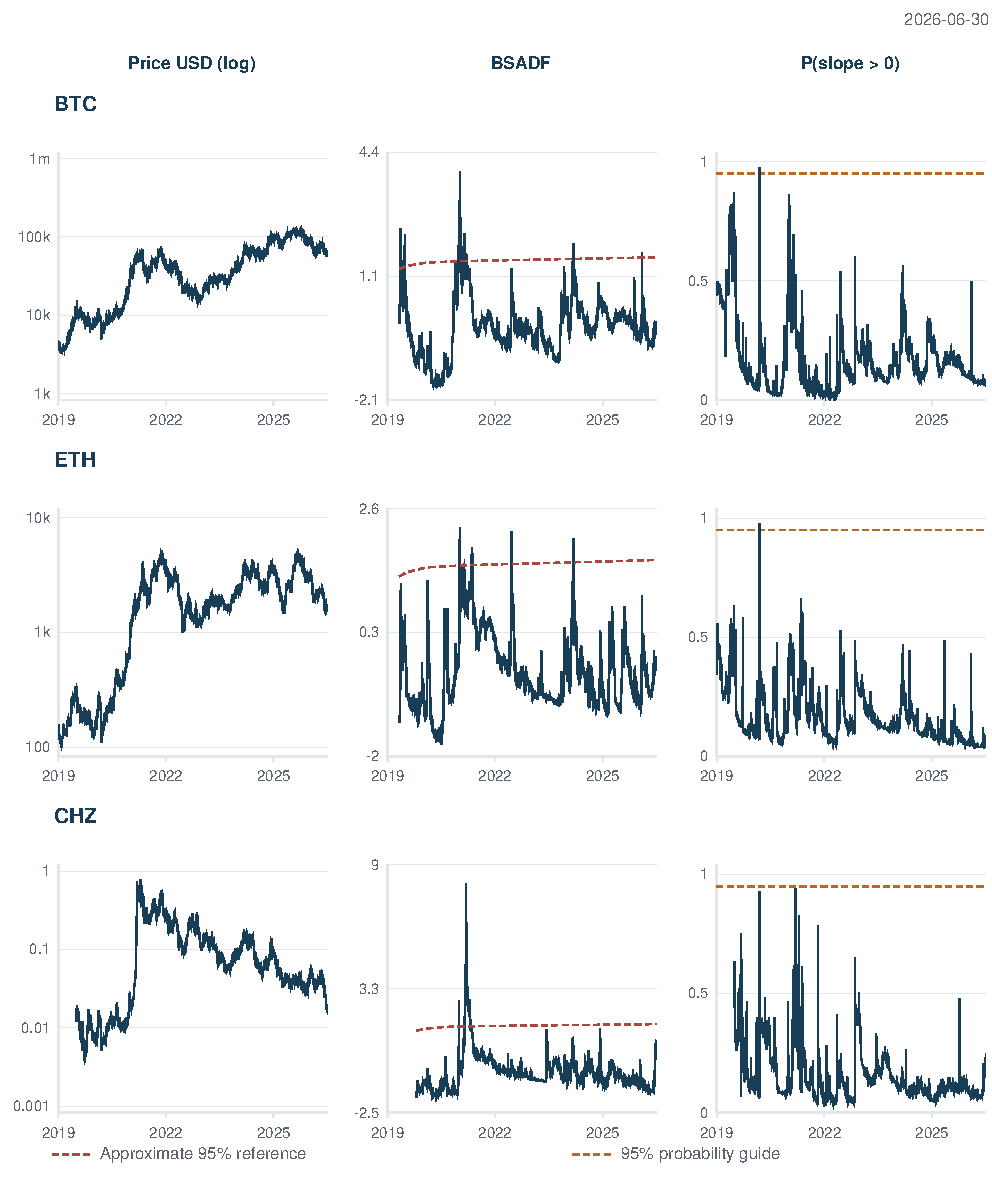
\includegraphics[width=\linewidth,height=.80\textheight,keepaspectratio]{figures/appendix/figure-A8.pdf}
\captionof{figure}{Figure A.8 BTC ETH and CHZ.}
\end{minipage}
\clearpage
\subsection{A.6 June and September comparisons}
\noindent\begin{minipage}{\linewidth}\centering
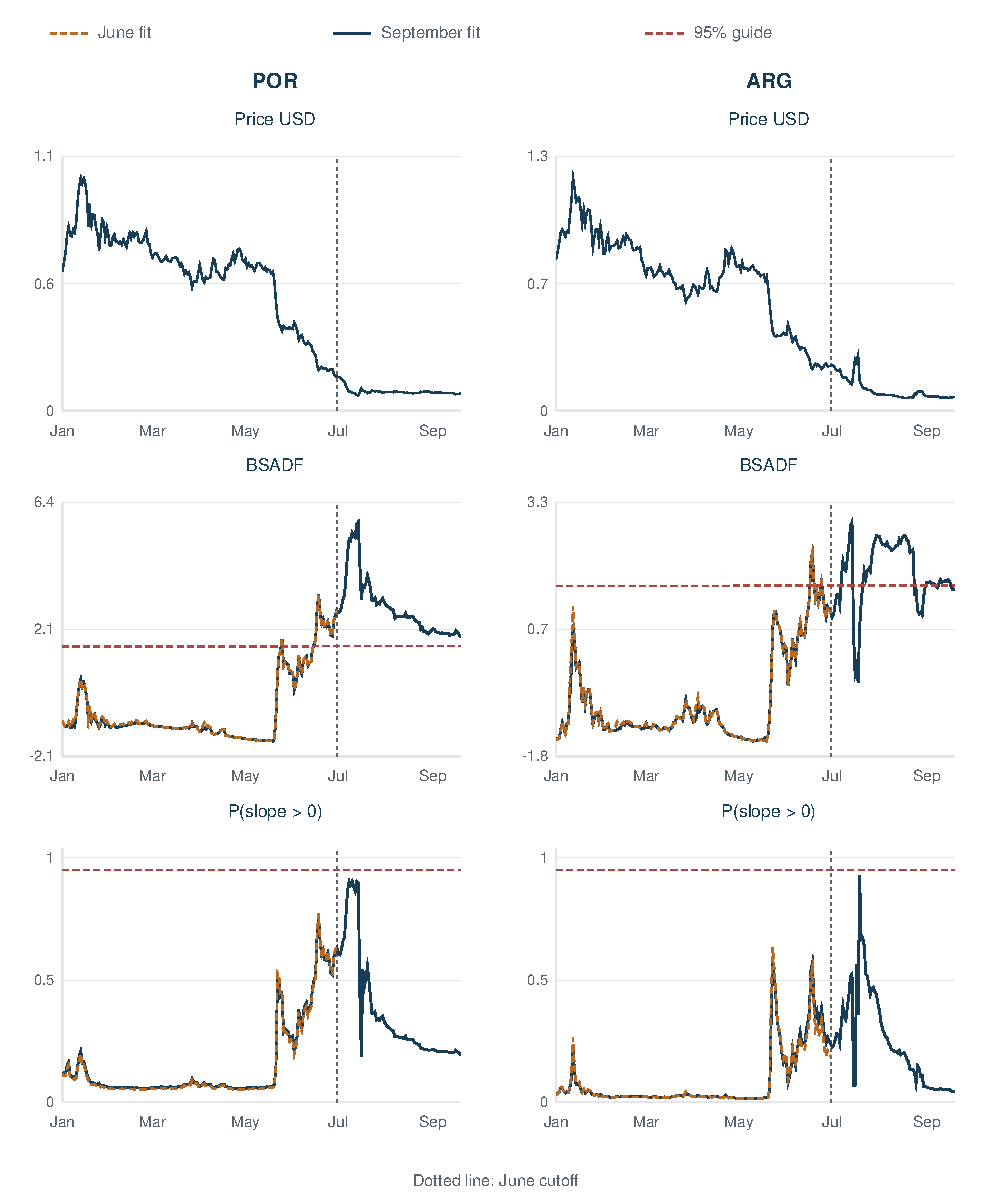
\includegraphics[width=\linewidth,height=.80\textheight,keepaspectratio]{figures/appendix/figure-A9.pdf}
\captionof{figure}{Figure A.9 POR and ARG.}
\end{minipage}
\end{document}